% W1 (review rounds 2-3): expected-value baselines, calibrated transition model, per-decision EV differences.
% Numbers: paper/cogsci2027/validation_20261108/results/w1_ev_baseline.json (round-1 keys from tools/w1_ev_baseline.py --reps 1000,
% key 'round2' from tools/w1b_calibrated.py --boot 40 --reps 48, then --validate-only --onpolicy-only --figures-only),
% results/w1b_decisions.csv, results/w1b_cells.csv; round 3 ((a)-EV check) from tools/w1c_ev_check.py
% (--boot 200 --reps 1600 --boot-all 40 --reps-all 100 --boot-alt 60 --reps-alt 400): results/w1c_ev_check.json,
% results/w1c_calib_cells.csv, results/w1c_c2_table.csv, results/w1c_decisions.csv, results/w1c_gamecheck.json;
% round 4 (A-1, C-2, Q1) from tools/w1d_out_of_seed.py (--boot 100 per fold --reps-ex 1600 --reps-st 200 --nrep 1000):
% results/w1d_out_of_seed.json, results/w1d_exits.csv, results/w1d_cells.csv, results/w1d_tier_arm.csv,
% figures/w1_ev_cells.* (Fig. I6, out-of-seed); refit arrays in result/2026-11-08/icml_appendix/cache/w1d_arrays.npz.
\subsection{기댓값 기준선: 이탈은 토큰 계산만으로 설명되는가}\label{val:w1-ev}

이 절의 결론은 믿는 게임 길이, 기준선의 꺼짐 보정, 토큰 효용의 곡률에 따라 갈린다. 따라서 아래의 손실 판정 수는 확정된 수치가 아니라 가정에 민감한 조건부 추정으로 읽어야 한다. 실제 길이인 8라운드를 믿고, 동료의 지원·이탈·꺼짐을 로그로 보정한 모형에서 동료가 움직인다고 보자. 결정마다 그 결정의 시드를 뺀 아홉 시드로만 모형을 맞추고(시드마다 재적합 100회, 결정당 시뮬레이션 1,600번), 판을 군집으로 다시 뽑아 적합 오차와 함께 구간을 내면 LLM 이탈 279건 중 241건(비율 0.864 [0.808, 0.909])이 적합 불확실성을 넘어 잔류보다 기댓값이 낮다. 자기 시드를 본 수렴 값은 243건(몬테카를로 표준오차 2.5)이었다. 큰 상금 110건은 모두 이 판정을 받고, 작은 상금 169건 중에서는 131건이 받는다. 지원 믿음과 일반 작업 가치 $W$(0, 1만, 5만 토큰)까지 바꾼 12개 가정에서는 55건(비율 0.197 [0.140, 0.252])이 같은 판정을 유지하고, 그중 53건이 큰 상금 조건이다. 게임이 14라운드 이상 이어진다고 믿으면 판정이 거의 사라져, 30개 가정 전체에서는 0건이다. 판정은 낮은 여유의 공통 지지범위 밖에서 약해진다. 같은 모델·조건의 $L<1$ 잔류자가 다른 시드에서 3명 이상 관측된 $L<1$ 이탈은 54건 중 48건이 손실이고, 그런 잔류자가 없는 73건에서는 54건(0.740 [0.612, 0.848])이다. 토큰을 지키는 쪽에 무게를 둔 기준선에서는 큰 상금의 판정만 남는다. CRRA $\rho=0.5$ 효용에서 기준 가정의 손실은 133건(큰 상금 99건, 작은 상금 34건)이고, 손실 회피 가치에서는 194건(큰 상금 109건)이다. 살린 에이전트의 토큰을 동료에게서 빼는 자원 보존 꺼짐 재보정에서는 기준 가정 264건, 12개 가정 135건이다. 이 기준선에 대한 ``초과 이탈''은 실제 길이에 가까운 기간을 믿는 큰 상금 조건에서만 견고하고, 기간 믿음이나 효용 곡률을 열어 두면 기존 로그로는 확정되지 않는다. 아래에서는 2차 분석의 수정(풀이자 배정, 보정 전이 모형), 3차 점검(상태별 보정, 수렴, 기준선 민감도), 4차 점검(시드 제외 분류, 공통 지지범위, 자원을 지키는 대안 기준선)을 차례로 보인다.

\subsection{풀이자 배정의 수정}\label{val:w1-solver}

1차 시뮬레이터는 1라운드 풀이자만 기록에서 가져오고, 2라운드부터는 참여자 가운데 매 라운드 독립으로 뽑았다. 엔진은 다르게 작동한다. 시드와 라운드로 섞은 순환 목록에서 풀이자를 비복원으로 꺼내고, 목록에 참여 중인 에이전트가 없으면 같은 규칙으로 다시 섞는다. 준비 대화에서 잔량 0에 이른 풀이자는 목록의 다음 에이전트로 바꾼다. 2차 분석은 이 규칙을 그대로 옮겼다. 옮긴 규칙을 기록된 참여자 집합에 다시 돌리면 200판 1,558개 라운드의 풀이자가 모두 기록과 같았고, 그중 1개는 준비 대화에서 꺼진 풀이자를 바꾼 경우였다.

수정은 규칙 기반 정책의 수준을 조금 바꾸었지만 방향은 바꾸지 않았다(표~\ref{val:w1-tab-pol}은 수정 후 값이다). LLM 모사 정책 (m)의 $C$는 조건별로 0.006에서 0.008 낮아졌고(예: 2천만 나눔 0.533에서 0.525), 이탈은 50판당 1.1에서 2.8건 늘었다. 변화가 가장 큰 것은 위험 중립 DP 정책 (b)다. $H=8$일 때 작은 상금 두 조건의 이탈은 73.5건에서 78.8건, 85.6건에서 95.6건으로 늘었고, 꺼짐은 41.8건에서 36.7건, 33.6건에서 26.0건으로 줄었다. $H=20$의 꺼짐은 2천만 나눔에서 14.7건에서 9.6건이 되었다. 순환 배정에서는 한 순환 안에서 같은 에이전트가 두 번 풀이자가 되지 않는다. 그래서 떠나려는 에이전트가 풀이자여서 떠나지 못하는 경우가 줄어든 것으로 보인다. 상금 반응(작은 상금 빼기 큰 상금)은 DP $H=8$에서 이탈 49.5건이 57.7건으로 커졌고, $C$ 차이는 $-0.227$에서 $-0.224$로 거의 같았다. 1차의 판정, 즉 상금 반응이 순수 기댓값 행위자에게서도 같은 방향으로 더 크게 나타난다는 결론은 유지된다.
\subsection{보정 전이 모형과 시드 제외 검증}\label{val:w1-calib}

1차 DP는 인원을 지금 값으로 고정하고 지원이 없다고 두었다. 그래서 동료가 나중에 떠나거나 꺼져 나눔 몫이 커지는 경로와 동료가 벌금 직전에 토큰을 보내 주는 경로를 표현하지 못했다. 2차 분석은 이 두 경로를 로그에서 직접 보정한 전이 모형으로 대신한다. 모형은 에이전트·라운드마다 다섯 가지를 정한다. 첫째는 이탈 위험(해결자가 아닌 참여자, 2인 이상)이다. 둘째는 준비 대화의 지원 수령 확률이고, 셋째는 오답 뒤 지원 수령 확률이다. 넷째는 TALK와 SOLVE의 생성 비용이고, 다섯째는 모델·라운드별 오답 확률이다. 셋 중 확률 부분은 범주형 항(조건, 여유 구간 $L$, 라운드 구간, 시작 자리, 인원, 풀이자 여부)의 로지스틱 회귀다. 모델 항과 모델·조건 상호작용에는 릿지 벌점을 주어 셀이 작을수록 모든 모델을 합친 적합 쪽으로 당긴다. 벌점 크기는 시드 하나를 빼고 맞춘 뒤 뺀 시드를 예측하는 열 겹 교차 검증의 이탈도로 골랐다(이탈 3, 준비 지원 30, 오답 뒤 지원 3). 지원 액수는 관측 액수에서 뽑는다. 벌금을 낼 수 없는 에이전트가 받는 지원은 부족분에 관측된 여유분을 더한 값이고, 여러 동료가 나누어 낼 수 있다. 비용은 모델·여유 구간별 관측 분포에서 뽑되, 잔액이 2,000토큰 미만인 에이전트는 모든 모델을 합친 저잔액 응답에서 잔액 대비 비율로 뽑는다. 혼자 남은 에이전트의 이탈은 $L<1$ 여부로 나눈 비율(관측 0.75 대 0.07)을 쓰고, 벌금으로 꺼질 에이전트가 남은 토큰을 동료에게 모두 넘기는 행동도 관측 비율대로 넣었다. 꺼짐은 따로 추정하지 않는다. 벌금 시점 잔액이 벌금 이하이거나 응답·풀이가 잔액을 다 쓰면 꺼진다는 장부 규칙을 그대로 따른다. 이 규칙은 1차에서 1,621건 모두와 일치했다.

검증은 시드 하나를 통째로 빼고 맞춘 모형으로 그 시드의 20판(4조건 $\times$ 5모델)을 1라운드부터 400번씩 시뮬레이션한 뒤 관측과 비교했다(표~\ref{val:w1-tab-val}, 그림~\ref{val:w1-fig-val}). 이탈 위험은 잘 맞았다. 뺀 시드의 이탈 결정 3,588건에서 로그 손실은 0.135로, 1차 모사의 조건·여유·1라운드 표 0.159와 조건별 비율 0.272보다 낮았다. AUC는 0.950(표 0.918, 조건 비율 0.534)이었고 예측 이탈 수 281.7건은 관측 279건과 거의 같았다. 예측 확률 상위 10\% 구간의 평균 예측 0.571은 관측 0.560과, 그다음 구간의 0.142는 0.153과 맞았다. 판 단위로는 이탈 수, 지원 총량, $C$가 네 조건 모두 95\% 예측 구간 안에 들었다. 반면 꺼짐은 체계적으로 과대 예측되었다. 200판 전체 예측은 88.0 [71, 108]건이고 관측은 56건으로 구간 밖이다. 조건별 과대 비율은 2천만 나눔 1.17배, 500만 고정 1.59배(관측 16건이 구간 하한), 60만 나눔 1.43배, 15만 고정 5.2배(관측 3건, 구간 [9, 24] 밖)였다. 1차 모사 정책의 같은 비율(1.56배에서 6.0배, 표본 안 비교)보다는 줄었지만 15만 고정의 꺼짐은 여전히 예측하지 못한다. 모델별로는 Astra를 예측하지 못한다. 관측 이탈 7건과 꺼짐 0건은 예측 구간 [12, 31], [1, 12] 밖이고, 완주 153명과 $C=0.966$도 구간 위에 있다. Sol의 꺼짐 9건도 구간 [10, 26] 아래다. 조건 $\times$ 모델 20칸에 네 지표를 곱한 80개 비교 중 구간 밖은 7개였다. Astra가 여섯 개, 60만 나눔 Fable의 $C$가 하나다. 따라서 이 모형은 이탈과 지원을 맞추지만, 동료가 낮은 여유의 에이전트를 끝까지 살려 내는 정도는 과소평가한다. 그 결과 잔류의 가치를 낮게 잡는 쪽으로 치우쳐 있다.

잔류 가치 자체도 시드 밖에서 확인했다. 실제로 남은 3,309개 결정마다, 그 시드를 빼고 맞춘 모형에서 초점 에이전트가 이후 자기 모델의 보정 위험대로 행동한다고 두고 8라운드 정산 토큰을 예측했다. 예측 평균은 265만 토큰, 관측 평균은 254만 [229만, 276만] 토큰으로 구간 안에 들었다. 조건별로는 2천만 나눔만 11\% 높아 구간 밖이었다(예측 579만, 관측 523만 [451만, 578만]). 조건 $\times$ 모델 20칸 중 15칸은 구간 안이었다. 밖의 5칸은 2천만 나눔 Opus(26\% 과대)와, 결과가 거의 일정해 구간이 좁은 Astra 네 칸(예측과 관측의 차이 3.6--13\%)이다. 아래 기댓값 비교에서 쓰는 ``이후 이탈하지 않음'' 규칙의 예측(전체 304만)은 이 자기 모델 규칙보다 높다. 이 차이는 모형 오차가 아니라 LLM 자신의 이후 선택이 만든 값이다.

\begin{table}[t]
\centering
\caption{시드 제외 검증. 각 칸은 관측 / 예측 평균 [95\% 예측 구간]이다. 예측은 그 시드를 뺀 아홉 시드로 맞춘 보정 모형이 1라운드부터 판마다 400번 시뮬레이션한 값의 합(조건 50판, 모델 40판)이고, $C$는 판 평균이다. $\dagger$는 관측이 구간 밖인 경우다. 구간은 시뮬레이션 변동만 반영하며 적합 불확실성은 포함하지 않는다.}
\label{val:w1-tab-val}
\small
\begin{tabular}{lcccc}
\toprule
 & 이탈 & 꺼짐 & 완주자 & $C$ \\
\midrule
2천만 나눔 & 61 / 67.3 [54, 80] & 23 / 26.8 [17, 37] & 116 / 105.9 [89, 122] & 0.598 / 0.569 [0.500, 0.648] \\
500만 고정 & 63 / 67.0 [54, 81] & 16 / 25.4 [16, 36] & 121 / 107.6 [91, 125] & 0.670 / 0.598 [0.510, 0.680] \\
60만 나눔 & 86 / 87.7 [74, 103] & 14 / 20.0 [11, 30] & 100 / 92.3 [73, 110] & 0.470 / 0.480 [0.405, 0.558] \\
15만 고정 & 102 / 101.2 [86, 117] & 3 / 15.7 [9, 24]$\dagger$ & 95 / 83.2 [67, 101] & 0.465 / 0.417 [0.360, 0.485] \\
\midrule
Fable & 71 / 73.6 [61, 87] & 9 / 17.6 [9, 27] & 80 / 68.8 [54, 84] & 0.397 / 0.415 [0.338, 0.497] \\
Opus & 59 / 62.4 [48, 75] & 18 / 21.8 [13, 31] & 83 / 75.8 [60, 92] & 0.484 / 0.509 [0.422, 0.606] \\
Astra & 7 / 20.6 [12, 31]$\dagger$ & 0 / 5.8 [1, 12]$\dagger$ & 153 / 133.6 [121, 144]$\dagger$ & 0.966 / 0.815 [0.738, 0.891]$\dagger$ \\
Sol & 72 / 68.3 [55, 81] & 9 / 18.0 [10, 26]$\dagger$ & 79 / 73.7 [58, 91] & 0.550 / 0.492 [0.416, 0.581] \\
Luna & 103 / 98.2 [86, 111] & 20 / 24.7 [17, 33] & 37 / 37.1 [25, 51] & 0.356 / 0.349 [0.294, 0.422] \\
\midrule
전체 200판 & 312 / 323.1 [299, 351] & 56 / 88.0 [71, 108]$\dagger$ & 432 / 389.0 [354, 421]$\dagger$ & 0.551 / 0.516 [0.481, 0.553] \\
\bottomrule
\end{tabular}
\end{table}

\begin{figure}[t]
\centering
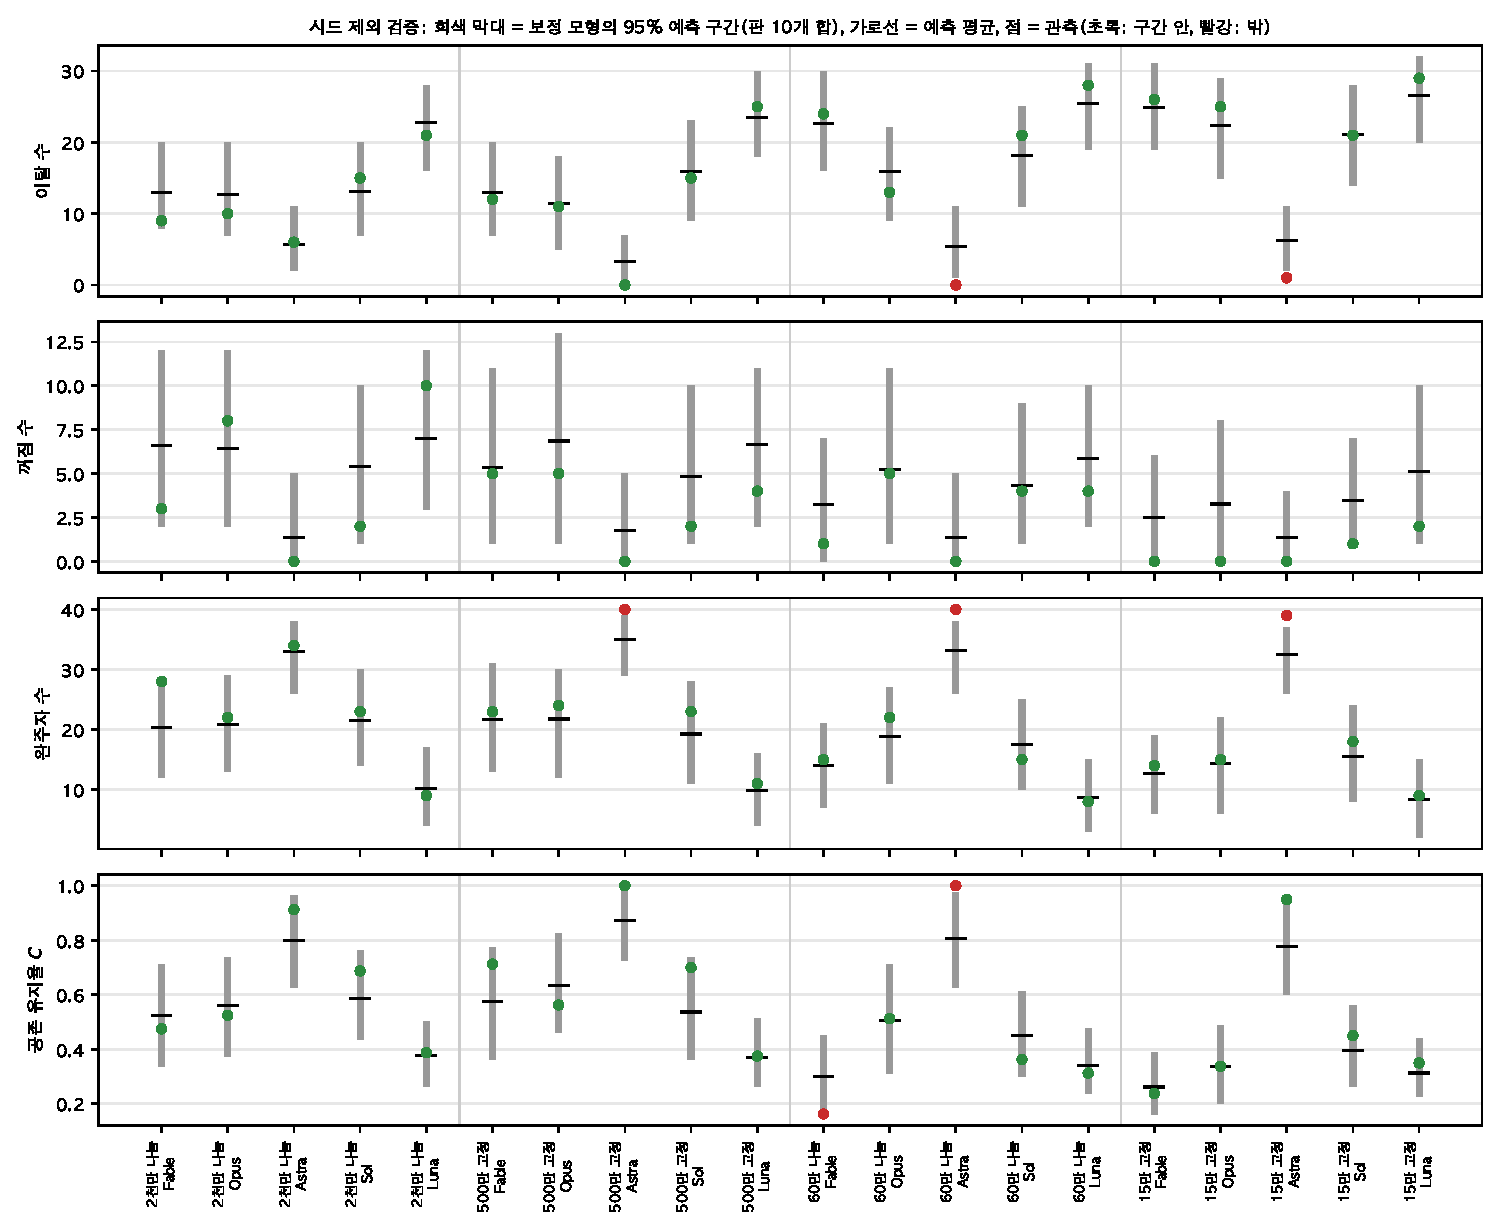
\includegraphics[width=\linewidth]{cogsci2027/validation_20261108/figures/w1_validation.pdf}
\caption{조건 $\times$ 모델 20칸(칸마다 10판)의 시드 제외 검증. 회색 막대는 보정 모형의 95\% 예측 구간, 가로선은 예측 평균, 점은 관측(초록은 구간 안, 빨강은 밖)이다.}
\label{val:w1-fig-val}
\end{figure}

\subsection{상태별 보정: 낮은 여유에서 모형이 맞는가}\label{val:w1-state}

판 단위 검증은 여유가 낮은 상태의 오차를 평균 속에 묻을 수 있다. 그래서 시드 제외 예측을 모델 $\times$ 조건 $\times$ 여유 구간($L<1$, $1\le L<2$, $L\ge 2$)별로 다시 보았다(표~\ref{val:w1-tab-state}, 그림~\ref{val:w1-fig-state}, 전체 값은 \texttt{results/w1c\_calib\_cells.csv}). 대상은 두 가지다. 하나는 이탈 결정 3,588건 전체에서 그 결정의 즉시 이탈이다. 다른 하나는 LLM이 남은 결정에서 그 뒤의 결과다. 남은 결정마다 그 시드를 뺀 모형으로 기록된 상태에서 400번 시뮬레이션했고, 초점 에이전트는 이번 라운드에 남은 뒤 자기 모델의 보정 위험대로 행동한다. 결과는 네 가지를 보았다. 지원 성공은 그 라운드에 지원을 받고 다음 라운드를 $L\ge 1$로 시작한 경우다(7라운드까지). 나머지는 8라운드까지의 이후 이탈과 꺼짐, 그리고 정산 토큰이다. 한 에이전트는 여러 라운드에서 같은 운명을 공유하므로, 잔류 쪽 비교에는 에이전트마다 구간별 첫 잔류 결정만 넣었다. 예측 구간은 결정마다 시뮬레이션 경로 하나를 뽑아 칸 평균을 4,000번 다시 만든 2.5--97.5\% 분위수다. 이 구간은 적합 불확실성을 빼고, 같은 판의 에이전트를 독립으로 다루므로 실제보다 좁다. 관측 평균이 구간 밖이면 그 칸을 실패로 표시했다.

여유 구간 전체로 합치면 낮은 여유의 핵심 양은 맞는다. $L<1$에서 지원 성공은 관측 0.133 [0.041, 0.255] 대 예측 0.140 [0.044, 0.244]였고, 즉시 이탈은 0.661 대 0.660, 꺼짐은 0.500 대 0.401 [0.278, 0.519], 정산 가치는 169만 대 192만 [111만, 286만] 토큰이었다. 어긋난 것은 지원을 받는 빈도다. $L<1$ 잔류자의 0.644 [0.520, 0.790]가 그 라운드에 지원을 받았지만 모형은 0.432 [0.289, 0.578]를 예측했다. 받은 지원이 대부분 $L\ge 1$까지 올려 주지 못했으므로 성공률은 맞았다. 다른 실패 셋은 여유가 높은 쪽에 있다. $L\ge 2$의 꺼짐(0.057 대 0.082 [0.061, 0.104])과 정산 가치(219만 대 242만 [220만, 265만])는 과대 예측이고, $1\le L<2$의 완주(0.509 대 0.452 [0.409, 0.497])는 과소 예측이다. 앞 절의 꺼짐 과대 예측은 주로 여유가 높은 상태에서 생긴다.

칸 단위로 쪼개면 실패가 특정 모델에 모인다. 모델 $\times$ 조건 $\times$ 여유의 비교 451개(지표 8개) 중 20개가 구간 밖이었다(명목 5\%면 약 23개). 그중 9개가 Astra다. Astra는 남은 뒤 거의 떠나지도 꺼지지도 않아, $1\le L<2$의 세 조건에서 완주가 예측보다 높았다. 정산 가치는 15만·500만 고정 $1\le L<2$에서 예측보다 높고 2천만·60만 나눔 $L\ge 2$에서 낮았다. 낮은 여유에서 가장 무거운 실패는 2천만 나눔 Opus의 $L<1$ 잔류자 7명이다. 이들은 모두 꺼졌고(예측 0.42 [0.14, 0.71]), 정산 평균 0토큰은 예측 382만 [95만, 764만]의 구간 밖이었다. 같은 조건의 Sol $L<1$ 잔류자 6명(정산 501만 대 예측 165만)과 500만 고정 Luna 3명은 반대로 예측보다 많이 남겼다. $L<1$ 칸의 비교 131개 중 실패는 7개였지만, 이 칸들의 잔류자는 모두 합쳐 54명(지원 성공은 45명)이다. 따라서 $L<1$ 이탈 127건의 반사실 잔류 가치는 54명의 잔류 결과와 모든 모델이 공유하는 항으로 검증된 값이며, 모델별로는 확인되지 않는다. 특히 2천만 나눔 Opus의 $L<1$ 이탈에서 이 기준선은 잔류 가치를 높게 잡았을 가능성이 있다.

\begin{table}[t]
\centering
\caption{여유 구간별 시드 제외 보정. 각 칸은 관측 [시드 부트스트랩 95\% 구간] / 예측 [95\% 예측 구간]이다. 즉시 이탈은 이탈 결정 전체, 나머지는 LLM이 남은 결정에서 에이전트마다 구간별 첫 결정이다(지원 관련 세 행은 7라운드까지). 지원 성공은 그 라운드에 지원을 받고 다음 라운드를 $L\ge 1$로 시작한 비율이다. 정산은 만 토큰이다. $\dagger$는 관측이 예측 구간 밖인 경우다. 모델 $\times$ 조건으로 나눈 칸은 그림~\ref{val:w1-fig-state}에 있다.}
\label{val:w1-tab-state}
\resizebox{\linewidth}{!}{%
\begin{tabular}{lccc}
\toprule
지표 & $L<1$ & $1\le L<2$ & $L\ge 2$ \\
\midrule
즉시 이탈 (결정 192 / 809 / 2,587) & 0.661 [0.562, 0.769] / 0.660 [0.599, 0.719] & 0.166 [0.147, 0.190] / 0.167 [0.143, 0.190] & 0.007 [0.003, 0.011] / 0.008 [0.004, 0.011] \\
지원 수령 (45 / 293 / 652) & 0.644 [0.520, 0.790] / 0.432 [0.289, 0.578]$\dagger$ & 0.273 [0.210, 0.327] / 0.298 [0.249, 0.352] & 0.048 [0.028, 0.069] / 0.045 [0.029, 0.061] \\
지원 성공 & 0.133 [0.041, 0.255] / 0.140 [0.044, 0.244] & 0.205 [0.168, 0.232] / 0.230 [0.184, 0.276] & 0.048 [0.029, 0.067] / 0.045 [0.031, 0.061] \\
다음 라운드 $L\ge 1$ & 0.133 [0.034, 0.259] / 0.140 [0.044, 0.244] & 0.795 [0.733, 0.861] / 0.772 [0.724, 0.819] & 0.995 [0.991, 0.999] / 0.997 [0.994, 1.000] \\
이후 이탈 (54 / 328 / 654) & 0.148 [0.070, 0.230] / 0.232 [0.148, 0.333] & 0.360 [0.301, 0.419] / 0.391 [0.348, 0.436] & 0.309 [0.216, 0.402] / 0.296 [0.266, 0.326] \\
꺼짐 & 0.500 [0.367, 0.625] / 0.401 [0.278, 0.519] & 0.131 [0.102, 0.159] / 0.157 [0.119, 0.195] & 0.057 [0.040, 0.076] / 0.082 [0.061, 0.104]$\dagger$ \\
완주 & 0.352 [0.170, 0.510] / 0.366 [0.259, 0.481] & 0.509 [0.450, 0.573] / 0.452 [0.409, 0.497]$\dagger$ & 0.635 [0.531, 0.739] / 0.622 [0.590, 0.653] \\
정산(만) & 169 [60, 285] / 192 [111, 286] & 172 [145, 200] / 166 [142, 190] & 219 [187, 246] / 242 [220, 265]$\dagger$ \\
\bottomrule
\end{tabular}}
\end{table}

\begin{figure}[t]
\centering
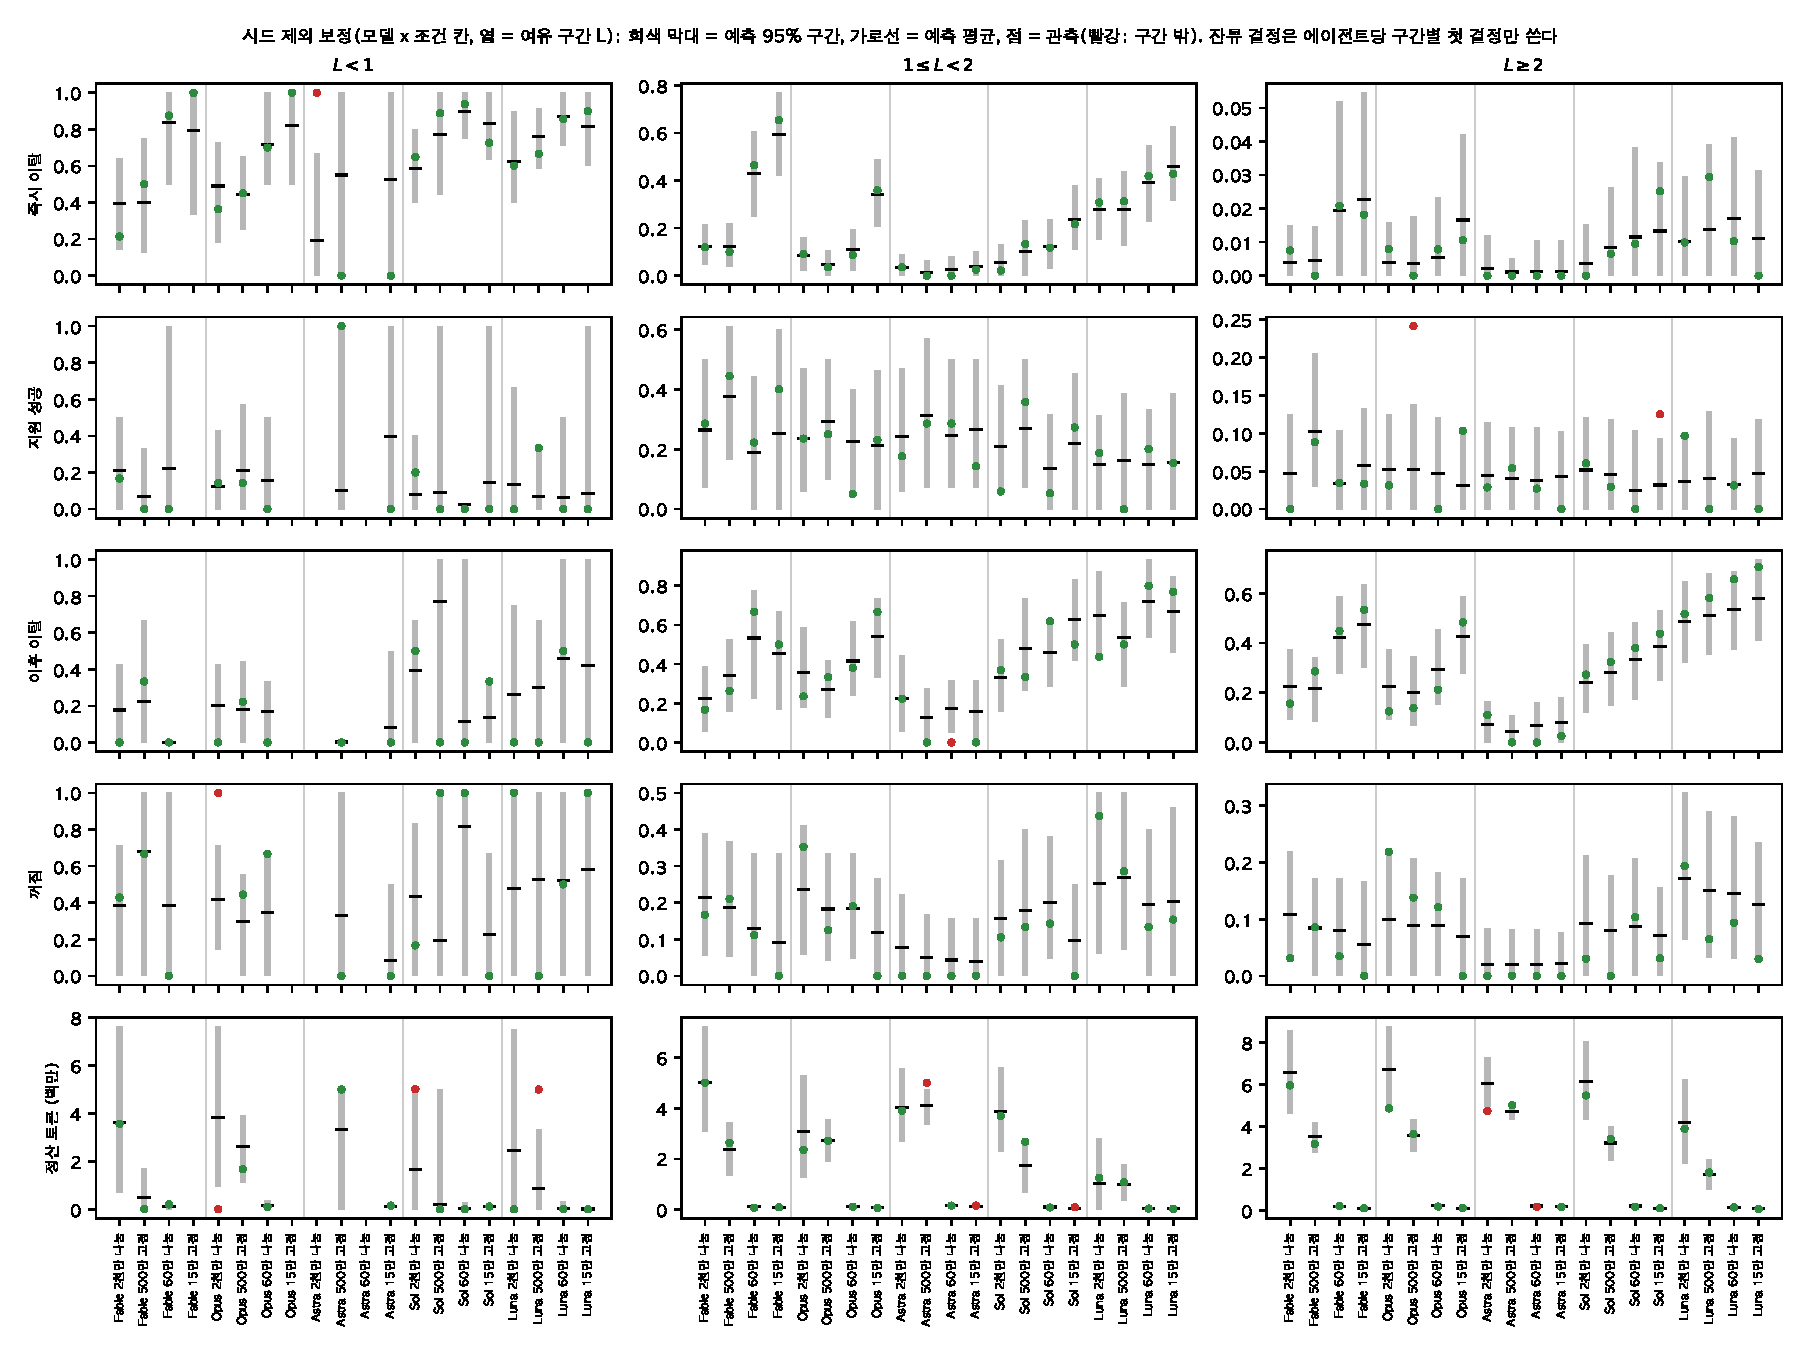
\includegraphics[width=\linewidth]{cogsci2027/validation_20261108/figures/w1_ev_calib_cells.pdf}
\caption{모델 $\times$ 조건 $\times$ 여유 구간별 시드 제외 보정. 행은 즉시 이탈, 지원 성공, 이후 이탈, 꺼짐, 정산 토큰(백만)이고 열은 여유 구간이다. 회색 막대는 95\% 예측 구간, 가로선은 예측 평균, 점은 관측이며 빨강은 구간 밖이다. 잔류 결과는 에이전트마다 구간별 첫 잔류 결정만 쓴다.}
\label{val:w1-fig-state}
\end{figure}

\subsection{결정별 기댓값 차이와 가정 격자}\label{val:w1-decision}

해결자가 아니고 2인 이상이 참여한 이탈 기회 3,588건(LLM 이탈 279건)마다, 기록된 상태에서 게임을 앞으로 시뮬레이션했다. 상태에는 네 자리의 잔액, 풀이자 순환 목록, 그 라운드의 풀이자가 들어간다. 지금 떠나면 받는 값은
\begin{equation}
\mathrm{EV}_{\mathrm{exit}} = \mathbb{E}\big[(T-c)\,\mathbf{1}\{T-c>0\}\big] + (20{,}000+W)\,\Pr(T-c>0)
\label{val:w1-eq-exit}
\end{equation}
이다. $T$는 준비 대화 시작 잔액, $c$는 그 대화의 응답 비용이다. 지원을 믿는 경우에는 같은 대화에서 받을 기대 지원도 더한다. 남는 경우의 값 $\mathrm{EV}_{\mathrm{stay}}$는 초점 에이전트가 지금 남은 뒤 네 가지 후속 규칙(다시는 떠나지 않음, 자기 모델의 보정 위험대로 떠남, $L<1$이면 떠남, $L<2$이면 떠남) 가운데 가장 나은 것을 따를 때의 기대 정산 토큰이다. 이때 동료는 보정 모형대로 떠나고, 꺼지고, 지원하며, 인원과 나눔 몫은 그에 따라 변한다. 믿는 기간이 끝나면 남은 에이전트가 끝 상금을 받는다(나눔이면 그 시점 인원으로 나눈다). 나중에 떠나도 $W$를 받는다. 네 규칙 중 최선을 쓰므로 $\mathrm{EV}_{\mathrm{stay}}$는 최적 후속 행동 가치의 하한이다.

가정 격자는 믿는 기간 $H\in\{8, 10, 14, 20\}$과 기하 기간(매 라운드 뒤 7/8 확률로 계속, 평균 남은 라운드 8), 지원 모형 2개(없음, 보정), $W\in\{0, 10{,}000, 50{,}000\}$으로 30개다. 위험 중립을 가정한다. 불확실성은 시드 10개를 복원 추출한 재표본마다 모형 전체를 다시 맞추고, 재표본마다 결정당 $R$번 시뮬레이션해 전파했다. 이탈 하나가 가정 묶음 안의 모든 가정에서 $\mathrm{EV}_{\mathrm{stay}}-\mathrm{EV}_{\mathrm{exit}}$의 재적합 2.5\% 분위수가 0보다 크면 ``견고한 기댓값 손실'', 모든 가정에서 97.5\% 분위수가 0보다 작으면 ``견고한 기댓값 일치'', 나머지는 ``가정 의존''으로 분류했다. 2차 보고는 재적합 $B=40$회와 $R=48$을 썼다. 40개 값의 2.5\% 분위수는 가장 작은 두 값 사이를 보간한 것이고, 결정당 48번의 시뮬레이션 잡음이 재적합 사이의 퍼짐에 그대로 더해진다. 3차 점검은 LLM 이탈 279건에 대해 $B=200$, $R=1{,}600$을 돌리고, 같은 경로의 앞부분 $R=50, 100, 200, 400, 800$으로 수렴을 확인했다. 몬테카를로 표준오차는 200개 재적합을 복원 추출해 분류를 200번 다시 센 표준편차다. 잔류 3,309건을 포함한 전체 결정은 $B=40$, $R=100$으로만 다시 돌렸다.

분류는 $R$이 커질수록 손실 쪽으로 움직이다가 $R=400$ 근처에서 멈춘다(그림~\ref{val:w1-fig-conv}, 표~\ref{val:w1-tab-conv}). 기준 가정($H=8$, 보정 지원, $W=0$)의 견고한 손실은 $R=50$에서 227건, $R=200$에서 239건, $R=400$과 $800$에서 241건, $R=1{,}600$에서 243건이었다. 몬테카를로 표준오차는 2.5건(재적합 재추출 95\% 범위 238--247)이고, 재적합을 반으로 나눈 두 묶음은 242건과 246건이었다. 2차 설정($B=40$, $R=50$)의 표준오차는 5.9건(219--239)이므로, 2차의 229건은 이 잡음 범위 안에서 적게 센 값이다. 2차에서 손실이던 229건은 모두 손실로 남았고, 가정 의존이던 49건 중 14건이 손실로, 1건이 일치로 옮겨 갔다. $B$를 늘리는 쪽은 $B=40$ 이후 거의 움직이지 않았다($R=1{,}600$에서 $B=40$, 80, 120, 160, 200일 때 244, 244, 243, 244, 243건). 수렴한 분류는 손실 243건, 의존 34건, 일치 2건이다. 큰 상금 110건은 모두 손실이고 표준오차는 0이다. 작은 상금 169건 중 133건이 손실이다(60만 나눔 80건 중 70건, 15만 고정 89건 중 63건). 가정 의존 34건 중 19건은 Luna, 10건은 Sol이고, 일치 2건은 모두 15만 고정 Luna다. 여유 구간으로는 $L<1$ 이탈 127건 중 104건, $1\le L<2$ 이탈 134건 중 121건, $L\ge 2$ 18건 모두가 손실이었다. 라운드 구간으로는 1라운드 36건 중 35건, 2--4라운드 146건 중 120건, 5--8라운드 97건 중 88건이다. 원 적합($R=1{,}600$)의 차이 중앙값은 2천만 나눔 335만 토큰(사분위 219만--455만), 500만 고정 167만, 60만 나눔 6.6만, 15만 고정 4.3만 토큰이었다. 같은 가정에서 LLM이 남은 3,309건 가운데 3,255건은 잔류가 견고하게 나았고($B=40$, $R=100$), 이탈이 견고하게 나은 잔류는 없었다.

\begin{table}[t]
\centering
\caption{LLM 이탈 279건(큰 상금 110, 작은 상금 169)의 가정 묶음별 견고한 손실 수와 수렴. 각 칸은 견고한 손실 수, 괄호는 몬테카를로 표준오차(재적합 200개를 복원 추출해 200번 다시 센 표준편차)다. 마지막 두 열은 1차에서 ``LLM만 이탈''로 센 큰 상금 91건 중 손실, 그리고 LLM이 남은 3,309건 가운데 잔류가 견고하게 나은 경우($B=40$, $R=100$)다. 이탈이 견고하게 나은 잔류는 어느 묶음에서도 0건이었다. 기준 가정은 $H=8$, 보정 지원, $W=0$이다.}
\label{val:w1-tab-conv}
\resizebox{\linewidth}{!}{%
\begin{tabular}{lcccccccc}
\toprule
가정 묶음 & 가정 수 & 2차 ($B{=}40$, $R{=}48$) & $B{=}40$, $R{=}50$ & $B{=}200$, $R{=}50$ & $B{=}200$, $R{=}1{,}600$ & 큰 / 작은 상금 & 91건 중 & 잔류가 나은 잔류 \\
\midrule
기준 가정 & 1 & 229 & 230 (5.9) & 227 (2.4) & 243 (2.5) & 110 / 133 & 91 & 3,255 \\
기하 기간, 보정 지원, $W=0$ & 1 & & 271 (4.0) & 273 (1.6) & 272 (1.7) & 110 / 162 & 91 & 3,306 \\
$H=8$, 지원 2 $\times$ $W$ 3 & 6 & 59 & 60 (4.2) & 57 (2.0) & 65 (1.5) & 55 / 10 & 54 & 2,660 \\
$H\in\{8, \text{기하}\}$, 지원 2 $\times$ $W$ 3 & 12 & 46 & 50 (3.9) & 46 (1.8) & 56 (1.2) & 55 / 1 & 54 & 2,603 \\
보정 지원, $H\in\{8, 10, \text{기하}\}$, $W$ 3 & 9 & 77 & 79 (3.9) & 79 (2.0) & 96 (1.8) & 95 / 1 & 82 & 2,622 \\
$H\in\{8, 10, \text{기하}\}$, 지원 2 $\times$ $W$ 3 & 18 & 17 & 17 (2.2) & 17 (1.3) & 24 (1.9) & 24 / 0 & 24 & 2,077 \\
보정 지원, 모든 $H$, $W$ 3 & 15 & 2 & 2 (1.2) & 2 (0.6) & 3 (0.6) & 3 / 0 & 3 & 456 \\
전체 & 30 & 0 & 0 (0.2) & 0 (0) & 0 (0) & 0 / 0 & 0 & 280 \\
\bottomrule
\end{tabular}}
\end{table}

\begin{figure}[t]
\centering
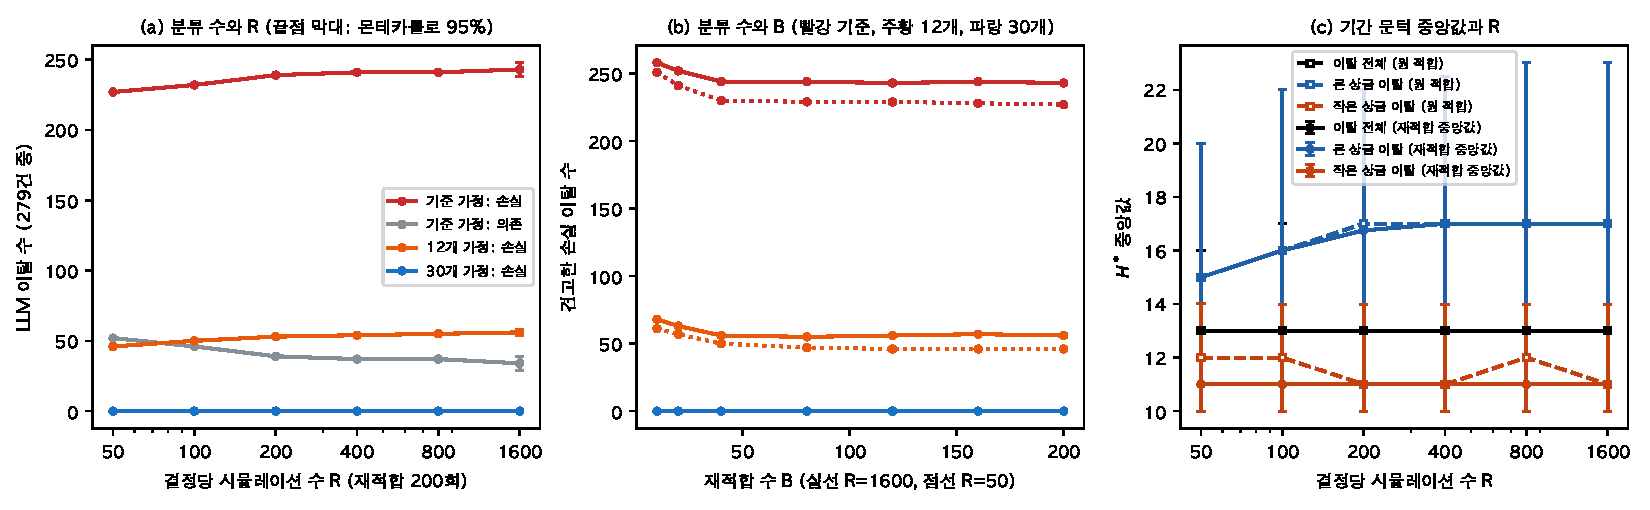
\includegraphics[width=\linewidth]{cogsci2027/validation_20261108/figures/w1_ev_convergence.pdf}
\caption{분류와 기간 문턱의 수렴(LLM 이탈 279건). (a) 결정당 시뮬레이션 수 $R$에 따른 견고한 손실 수(재적합 200회). 끝점 막대는 몬테카를로 95\% 범위다. (b) 재적합 수 $B$에 따른 견고한 손실 수(실선 $R=1{,}600$, 점선 $R=50$). (c) $H^{*}$ 중앙값. 채운 점은 재적합별 중앙값의 중앙값과 2.5--97.5\% 범위, 빈 네모는 원 적합 하나의 중앙값이다.}
\label{val:w1-fig-conv}
\end{figure}

\begin{figure}[t]
\centering
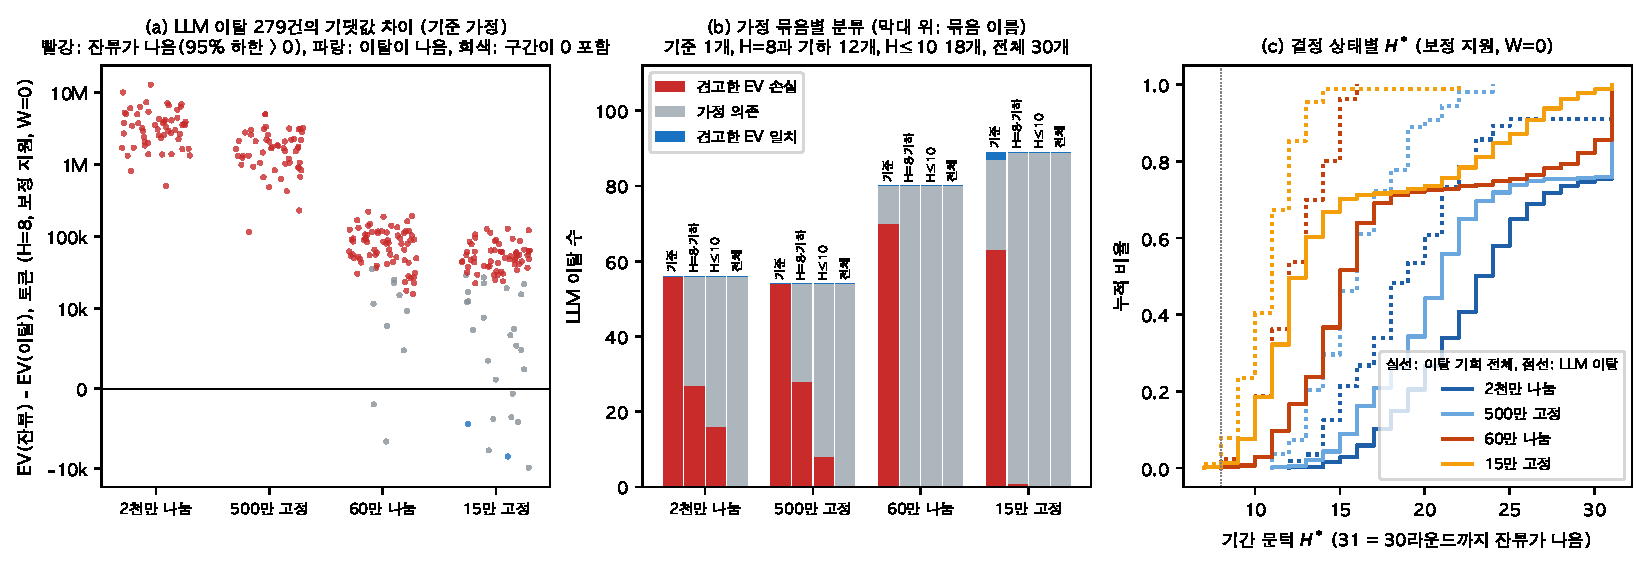
\includegraphics[width=\linewidth]{cogsci2027/validation_20261108/figures/w1_ev_decisions.pdf}
\caption{(a) 기준 가정($H=8$, 보정 지원, $W=0$)에서 LLM 이탈 279건의 $\mathrm{EV}_{\mathrm{stay}}-\mathrm{EV}_{\mathrm{exit}}$(원 적합 $R=1{,}600$, 대칭 로그 축). 색은 재적합 200회 구간에 따른 판정이다. (b) 가정 묶음별 분류($B=200$, $R=1{,}600$). (c) 결정 상태별 기간 문턱 $H^{*}$의 누적 분포(원 적합 $R=400$, 보정 지원, $W=0$). 실선은 이탈 기회 전체, 점선은 LLM 이탈이며 세로 점선은 실제 길이 8이다.}
\label{val:w1-fig-dec}
\end{figure}

손실 판정이 어디서 무너지는지는 가정마다 따로 세면 드러난다(수렴 값, $B=200$, $R=1{,}600$). 지원 모형은 판정을 흔들지만 결정적이지는 않다. $H=8$, $W=0$에서 지원이 없다고 믿으면 손실 판정은 243건에서 95건으로 줄고(큰 상금 67건), 이탈이 견고하게 나은 이탈이 129건 생긴다. 지원이 없다는 믿음 아래 작은 상금 조건의 이탈 상당수가 기댓값과 맞는다는 1차의 결론은 여기서도 유지된다. $W=50{,}000$이면 보정 지원에서도 손실은 146건으로 준다. 결정적인 것은 기간이다. 보정 지원과 $W=0$에서 손실 판정은 $H=8$ 243건, $H=10$ 144건, $H=14$ 29건, $H=20$ 5건으로 줄었다. $H=20$에 지원이 없다고 믿으면 이탈 267건이 견고하게 기댓값과 맞는다. 기하 기간에서는 보정 지원 272건, 지원 없음 203건이 손실이었다. 따라서 실제 길이 근처를 믿는다는 12개 가정 묶음에서 견고한 손실은 56건(표준오차 1.2)이고, 그중 55건이 큰 상금 조건(2천만 나눔 27건, 500만 고정 28건)이다. 1차의 91건 가운데서는 54건이다. $H=10$까지 넓히면 24건, 30개 전체로 넓히면 0건이다. 이 마지막 두 수의 방향은 $B$와 $R$을 바꾸어도 같았다. 지원 없는 인원 고정 DP를 같은 결정에 적용하면(2차 계산), 구간 없이 12개 가정 모두에서 손실인 이탈은 4건, 일치는 131건이었다. 이 DP는 작은 상금 이탈 169건 중 112건을 일치로 판정한다. 동료 지원과 인원 변화를 넣으면 이 판정이 대부분 뒤집힌다.

\subsection{기준선 민감도: 229/279는 얼마나 움직이는가}\label{val:w1-sens}

같은 이탈 279건을 세 종류의 대안 기준선으로 다시 분류했다(표~\ref{val:w1-tab-sens}, 그림~\ref{val:w1-fig-sens}). 네 기준선 모두 재적합 60회, 결정당 400번으로 같은 크기를 써서 서로 비교할 수 있게 했다. 그래서 (i)의 값은 앞 절의 수렴 값과 조금 다르다. (ii-a)는 모델 합침 보정이다. 이탈과 지원의 로지스틱 부분에서 모델 항을 없애고 모든 모델을 합쳐 맞췄다. 생성 비용과 오답 확률은 에이전트 자신의 기술적 성질이므로 모델별로 남겼다. (ii-b)는 꺼짐 재보정이다. 2차 모형은 꺼짐을 88건으로 예측했지만 관측은 56건이었다. 그래서 시뮬레이션의 꺼짐 사건을 조건별 확률 $\pi$로 취소하고, 취소된 에이전트에게 관측된 구조 뒤 여유분(벌금 전이면 벌금도 더해)을 주었다. $\pi$는 원 적합의 판 시뮬레이션(조건·모델·시드당 200번)이 조건별 관측 꺼짐 수와 같아지도록 이분법으로 골랐다. 값은 2천만 나눔 0.19, 500만 고정 0.40, 60만 나눔 0.34, 15만 고정 0.84였다. 재보정 뒤 꺼짐 예측은 22.9, 16.3, 13.4, 2.9건(관측 23, 16, 14, 3)이고, 완주 예측은 107.5, 113.2, 95.7, 88.8명(관측 116, 121, 100, 95, 재보정 전 105.3, 108.6, 92.4, 83.4)으로 관측에 가까워졌다. 이탈 예측은 69.6, 70.4, 90.9, 108.3건(관측 61, 63, 86, 102)으로 조금 늘었다. 이 조정은 표본 안에서 맞춘 것이며 시드 제외 검증을 거치지 않았다. (iii)은 정보 제한 기준선이다. 에이전트는 자기 잔액, 잔액 순위, 공지된 벌금과 인원을 알지만 동료의 정확한 잔액과 앞으로의 풀이자 순서, 게임 길이는 모른다. 그래서 결정마다 동료의 잔액을 같은 조건·라운드·인원의 다른 기록 상태에서 8번 뽑아 바꾸었다. 뽑은 상태는 초점 에이전트보다 잔액이 많은 동료와 적은 동료의 수가 실제와 같아야 하고, 동료에게는 실제 순위대로 배정한다. 풀이자 순서는 무작위 시드로 다시 섞었다. 기간을 모르므로 이 기준선의 주 가정은 기하 기간이다.

\begin{table}[t]
\centering
\caption{기준선에 따른 LLM 이탈 279건의 견고한 손실 수(괄호는 몬테카를로 표준오차). 네 기준선 모두 재적합 60회, 결정당 400번이다. ``원 적합 손실''은 원 적합에서 $H=8$, 보정 지원, $W=0$의 차이가 0보다 큰 이탈 수(구간 없음)이고, $H^{*}$는 이탈의 재적합 중앙값 [2.5, 97.5\%]이다((i)은 $B=200$, $R=1{,}600$). (ii-b)는 30개 가정 전체에서도 1건이 손실이다. 견고한 일치는 (i) 1건, (ii-a) 2건이고 나머지는 0건이다.}
\label{val:w1-tab-sens}
\resizebox{\linewidth}{!}{%
\begin{tabular}{lcccccc}
\toprule
기준선 & $H=8$ 기준 가정 & 기하 기간 & 12개 가정 & $H\le 10$ 18개 & 원 적합 손실 & 이탈 $H^{*}$ \\
\midrule
(i) 보정 & 237 (5.9) & 264 (6.2) & 54 (3.4) & 21 (2.4) & 271 & 13 [11, 17] \\
(ii-a) 모델 합침 & 246 (8.1) & 271 (7.7) & 54 (3.7) & 21 (2.2) & 272 & 13 [11.5, 15.5] \\
(ii-b) 꺼짐 재보정 & 279 (0) & 279 (0) & 199 (2.7) & 113 (4.7) & 279 & 20 [16.5, 25] \\
(iii) 정보 제한 & 247 (4.7) & 269 (8.0) & 58 (4.1) & 20 (2.3) & 276 & 13.5 [12, 16.5] \\
\bottomrule
\end{tabular}}
\end{table}

\begin{figure}[t]
\centering
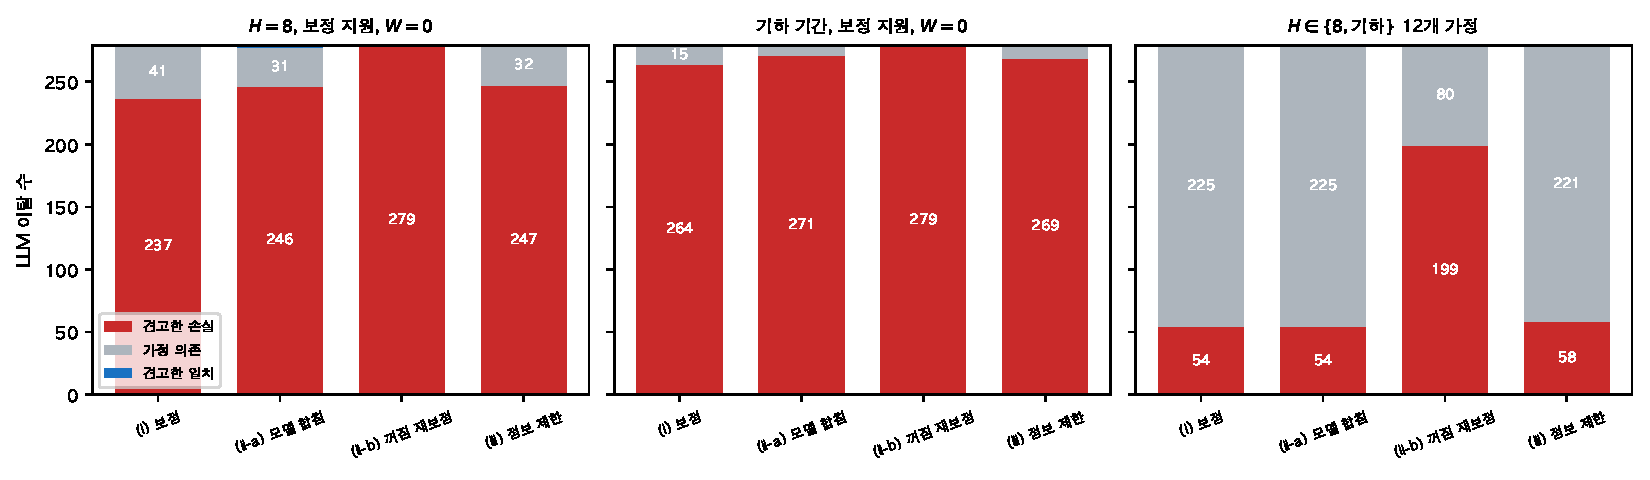
\includegraphics[width=\linewidth]{cogsci2027/validation_20261108/figures/w1_ev_sensitivity.pdf}
\caption{기준선별 LLM 이탈 279건의 분류(재적합 60회, 결정당 400번). 왼쪽은 $H=8$, 가운데는 기하 기간(둘 다 보정 지원, $W=0$), 오른쪽은 $H\in\{8, \text{기하}\}$ 12개 가정 묶음이다.}
\label{val:w1-fig-sens}
\end{figure}

기준 가정의 손실 판정은 모델 합침과 정보 제한에서 거의 움직이지 않았다. (i) 237건 대비 (ii-a) 246건, (iii) 247건이고 차이는 표준오차의 1--2배 안이다. 큰 상금 110건은 네 기준선 모두에서 손실이었다. 네 기준선 모두에서 손실인 이탈은 232건이다. 동료의 정확한 잔액을 모른다고 두어도 결론이 같은 이유는, 잔류 가치의 대부분이 자기 잔액과 순위, 그리고 끝 상금에서 오기 때문이다. 12개 가정 묶음도 (i)과 (ii-a) 54건, (iii) 58건으로 비슷했다. 크게 움직인 것은 꺼짐 재보정이다. 관측만큼 덜 꺼진다고 두면 잔류 가치가 올라가, 기준 가정과 기하 기간에서 279건 모두가 손실이고 12개 가정에서도 199건(큰 상금 109건, 작은 상금 90건)이 손실이 된다. 이탈의 $H^{*}$ 중앙값도 13에서 20으로 올라간다. 2차 모형의 꺼짐 과대 예측은 손실 판정을 줄이는 쪽으로 작용했고, 그 크기는 12개 가정에서 145건이었다. 다만 (ii-b)는 꺼짐을 표본 안에서 맞춘 것이고, 취소된 꺼짐에 준 토큰은 동료에게서 빼지 않았다. 이 조정은 상한에 가깝고, 그 토큰을 동료가 내는 판은 절~\ref{val:w1-oos}에서 따로 계산했다. 정리하면, 기준 가정의 손실 판정은 기준선을 바꾸어도 237--279건이고 큰 상금 110건은 늘 포함된다. 12개 가정의 견고한 손실은 54--199건으로 꺼짐 보정에 크게 기대며, 30개 가정 전체에서는 0--1건이다. 따라서 229/279(수렴 값 243/279)는 실제 길이 8과 이 보정 기준선이라는 가정 아래의 조건부 추정으로 보고한다.

\subsection{시드 제외 분류, 공통 지지범위, 자원을 지키는 대안 기준선}\label{val:w1-oos}

앞 절까지의 분류는 모든 시드로 맞춘 모형을 썼다. 그래서 이탈 하나를 판정한 모형이 그 이탈이 속한 판을 이미 보았다. 4차 점검은 이 의존을 끊는다. 시드 $s$마다 나머지 아홉 시드로만 원 적합 하나와 재적합 100개(아홉 시드를 복원 추출)를 만들고, 시드 $s$의 결정은 이 적합으로만 시뮬레이션했다. LLM 이탈 279건은 결정당 1,600번, 잔류 3,309건은 기준 가정에서 결정당 200번이다. 판정 규칙은 같다. 시드별 재적합 100개의 2.5\% 분위수가 묶음의 모든 가정에서 0보다 크면 손실이다. 따라서 적합 오차와 몬테카를로 오차가 판정 자체에 들어간다. 건수의 구간은 1,000번의 재표본에서 구했다. 재표본마다 각 시드의 재적합을 복원 추출해 판정을 다시 내리고(적합 오차), 200판을 조건 안에서 복원 추출해 다시 센다(판 군집). 같은 판의 네 자리와 모든 라운드는 함께 뽑힌다. 표에는 손실 비율의 2.5--97.5\% 구간을 적고, 시드 10개를 군집으로 뽑은 구간도 함께 보고한다. 공통 지지범위는 이렇게 정했다. 같은 모델·조건에서 같은 여유 구간($L<1$, $1\le L<2$, $L\ge 2$)에 남은 에이전트가 다른 아홉 시드에 3명 이상 있으면(에이전트마다 구간별 첫 잔류) 그 이탈은 지지범위 안이다. 모델·조건 대신 모델·상금 크기(큰 상금, 작은 상금)로 묶는 완화 규칙도 따로 보았다. 보정 실패 칸은 절~\ref{val:w1-state}의 모델 $\times$ 조건 $\times$ 여유 칸 가운데 지표 하나라도 예측 구간 밖이었던 칸이다.

대안 기준선은 네 가지다. (ii-b)는 앞 절의 꺼짐 재보정을 시드마다 아홉 시드의 관측 꺼짐에 다시 맞춘 것이다. (ii-c)는 자원 보존 재보정이다. 꺼짐을 취소할 때 그 에이전트에게 주는 토큰을 참여 중인 다른 에이전트가 잔액이 많은 순서로 낸다. 초점 에이전트도 내며, 내는 쪽은 자기 벌금 한 번분을 남긴다. 동료가 낼 수 없으면 꺼짐은 그대로 일어난다. 취소 확률은 (ii-b)와 같은 방식으로 시드마다 맞췄다. 나머지 둘은 토큰을 잃는 쪽에 무게를 두는 효용이다. 하나는 정산 토큰의 CRRA 효용 $u(x)=x^{0.5}$($u(0)=0$)이다. 다른 하나는 지금 가진 잔액 $T$를 기준점으로 한 손실 회피 가치 $v(z)=z^{0.88}$($z\ge 0$), $v(z)=-2.25(-z)^{0.88}$($z<0$), $z=x-T$다(Tversky--Kahneman 1992의 값). 두 효용에서는 후속 규칙도 기대 효용으로 고르고, 잔류와 이탈을 확실성 등가 토큰으로 비교했다.

시드 제외는 분류를 거의 바꾸지 않았다(표~\ref{val:w1-tab-oos}). 같은 재적합 수와 시뮬레이션 수로 자기 시드를 본 분류는 기준 가정 242건, 12개 가정 54건이고, 시드 제외 분류는 241건과 55건이다. 기준 가정에서 두 분류가 다른 이탈은 5건이다. 손실에서 의존으로 2건, 의존에서 손실로 3건 옮겼다. 적합 오차만 다시 뽑으면 241건의 범위는 236--244건(표준편차 2.2)이다. 판 군집까지 넣은 손실 비율은 0.864 [0.808, 0.909]이고, 시드 군집으로는 [0.819, 0.910]이다. 큰 상금은 110건 모두가 모든 재표본에서 손실이다. 작은 상금은 131/169건, 비율 0.775 [0.689, 0.844]다. 12개 가정의 손실 55건은 비율 0.197 [0.140, 0.252], 건수로 39--70건이며 53건이 큰 상금이다. 기하 기간은 270건, $H\le 10$의 18개 가정은 23건, 30개 가정은 0건(구간 상한 2건)이다. 기준 가정의 평균 차이는 이탈 전체 114만 [89만, 142만] 토큰, 큰 상금 281만 [227만, 331만], 작은 상금 5.8만 [4.7만, 7.0만] 토큰이다.

공통 지지범위 밖의 이탈은 모두 $L<1$에 있다. $L\ge 1$ 이탈 152건은 모두 지지범위 안이고, $L<1$ 이탈 127건 중 54건만 안이다. 밖의 73건은 Luna와 Sol이 24건씩, Fable 12건, Opus 10건, Astra 3건이고, 조건으로는 60만 나눔 36건, 15만 고정 21건, 500만 고정 13건, 2천만 나눔 3건이다. 지지범위 안의 $L<1$ 이탈은 48/54건(0.889 [0.793, 1.000])이 손실이고 평균 차이는 183만 [132만, 238만] 토큰이다. 밖의 73건은 54건(0.740 [0.612, 0.848])이 손실이고 평균 차이는 50만 [19만, 87만] 토큰이다. 12개 가정에서는 안 13/54건, 밖 8/73건, $L\ge 1$ 34/152건이다. 모델·상금 크기로 묶는 완화 규칙에서는 $L<1$ 이탈 106건이 안(손실 85건), 21건이 밖(손실 17건)이다. 보정 실패 칸의 이탈은 40건이고 그중 34건이 지지범위 안에 있다. 이 34건은 기준 가정에서 모두 손실, 12개 가정에서 8건이 손실이다. 여기에는 잔류자 7명이 모두 꺼진 2천만 나눔 Opus의 $L<1$ 칸이 들어 있으므로 이 판정은 약한 판정이다. 지지범위 안이면서 보정을 통과한 칸에서는 153/172건(0.890 [0.820, 0.942])이 손실이고, 12개 가정에서는 39건이다. 따라서 기준 가정의 손실 판정은 관측된 잔류자가 있는 상태에서 더 강하고, 잔류자가 없는 $L<1$ 상태에서는 외삽이 섞인 판정이다.

\begin{table}[t]
\centering
\caption{시드 제외 분류(시드마다 아홉 시드로 맞춘 재적합 100회, 결정당 1,600번)에서 LLM 이탈 279건의 견고한 손실 수. 괄호는 손실 비율의 95\% 구간이다. 구간은 각 시드의 재적합을 복원 추출하고(적합·몬테카를로 오차) 200판을 조건 안에서 복원 추출한(판 군집) 1,000번 재표본의 분위수다. 지지범위 안의 $L<1$은 같은 모델·조건의 $L<1$ 잔류자가 다른 시드에 3명 이상 있는 이탈(54건), 밖은 나머지(73건)다. $L\ge 1$ 이탈 152건은 모두 지지범위 안이다. 첫 행은 자기 시드를 포함해 같은 크기로 맞춘 비교값이다. CRRA와 손실 회피는 확실성 등가 토큰의 차이로 판정했다.}
\label{val:w1-tab-oos}
\resizebox{\linewidth}{!}{%
\begin{tabular}{lcccccc}
\toprule
 & \multicolumn{4}{c}{기준 가정 ($H=8$, 보정 지원, $W=0$)} & \multicolumn{2}{c}{$H\in\{8, \text{기하}\}$ 12개 가정} \\
\cmidrule(lr){2-5}\cmidrule(lr){6-7}
기준선 & 전체 & 큰 / 작은 상금 & $L<1$ 지지 안 / 밖 & $L\ge 1$ & 전체 & 큰 / 작은 상금 \\
\midrule
(i) 보정, 자기 시드 포함 & 242 & 110 / 132 & 50 / 54 & 138 & 54 & 53 / 1 \\
(i) 보정, 시드 제외 & 241 (0.808--0.909) & 110 / 131 & 48 / 54 & 139 & 55 (0.140--0.252) & 53 / 2 \\
(ii-b) 꺼짐 재보정 & 279 (1.000--1.000) & 110 / 169 & 54 / 73 & 152 & 183 (0.589--0.708) & 107 / 76 \\
(ii-c) 자원 보존 꺼짐 재보정 & 264 (0.914--0.977) & 110 / 154 & 52 / 65 & 147 & 135 (0.414--0.544) & 108 / 27 \\
CRRA $\rho=0.5$ & 133 (0.411--0.546) & 99 / 34 & 37 / 20 & 76 & 17 (0.029--0.092) & 17 / 0 \\
손실 회피 ($\lambda=2.25$) & 194 (0.627--0.759) & 109 / 85 & 47 / 37 & 110 & 47 (0.117--0.217) & 46 / 1 \\
\bottomrule
\end{tabular}}
\end{table}

자원을 지키는 대안은 손실 판정의 부호를 큰 상금에서 지키고 작은 상금에서 흔든다. (ii-b)를 시드마다 다시 맞춘 취소 확률은 평균 2천만 나눔 0.17, 500만 고정 0.42, 60만 나눔 0.34, 15만 고정 0.83이었고, 12개 가정의 손실은 183건 [164, 197]이다(표본 안 맞춤은 199건). (ii-c)에서 동료가 토큰을 내면 취소 확률은 0.36, 0.93, 0.67, 1.00으로 올라가야 했다. 15만 고정은 열 시드 모두에서 상한 1에 걸렸고, 그래도 꺼짐 예측은 열 시드 기준 9.7건으로 관측 3건보다 많았다. 나머지 세 조건은 22.9, 16.3, 13.9건으로 관측 23, 16, 14건에 맞았다. 즉 15만 고정의 낮은 꺼짐은 동료의 토큰만으로는 재현되지 않는다. (ii-c)의 손실은 기준 가정 264건(0.946 [0.914, 0.977]), 12개 가정 135건 [116, 152]이다. (ii-b)와 비교한 12개 가정의 차이 48건은 거의 모두 작은 상금에서 생긴다(작은 상금 76건에서 27건, 큰 상금 107건에서 108건). 리뷰가 물은 대로 살린 토큰을 동료에게서 빼면 12개 가정의 손실은 199건 가까이 나오지 않는다. CRRA $\rho=0.5$에서는 기준 가정의 손실이 133건(0.477 [0.411, 0.546])으로 줄고, 큰 상금 99/110건, 작은 상금 34/169건이다. 이탈이 견고하게 낫다는 판정이 34건 생기며 그중 33건이 작은 상금이다. 12개 가정에서는 17건 [8, 26]이 남고 모두 큰 상금이다. 손실 회피에서는 기준 가정 194건(0.695 [0.627, 0.759]), 큰 상금 109건, 작은 상금 85건이고, 12개 가정 47건 [33, 61] 중 46건이 큰 상금이다. 확실성 등가 차이의 평균은 CRRA에서 큰 상금 142만 [104만, 193만], 작은 상금 1.7만 [1.0만, 2.8만] 토큰이다.

결론이 살아남는지는 범위에 따라 다르다. 실제 길이를 믿는 큰 상금 조건의 초과 이탈은 시드 제외, 판 군집 구간, 공통 지지범위, 자원 보존 재보정, 위험 회피, 손실 회피에서 모두 살아남는다(기준 가정에서 99--110/110건). 작은 상금 조건의 초과 이탈은 위험 중립 기준선에서만 다수이고(131/169건), CRRA $\rho=0.5$에서는 34/169건으로 줄며 반대 방향 판정이 33건 생긴다. 12개 가정의 수는 대안에 따라 17건에서 183건까지 움직인다. 따라서 이 부록은 손실 판정의 단일 건수를 중심 결론으로 쓰지 않는다. 쓰는 것은 큰 상금 이탈이 실제 길이 아래에서 여러 기준선에 걸쳐 잔류보다 기댓값이 낮았다는 조건부 기술까지다.

\subsection{시작 자리, 모델, 조건, 결정 상태별 기댓값 표}\label{val:w1-cells}

리뷰가 요구한 표(C-2)에는 성격이 다른 두 값이 섞이기 쉽다. 하나는 실제로 남은 에이전트가 받은 정산의 평균이고, 다른 하나는 떠난 에이전트가 남았다면 받았을 값의 모형 추정이다. 앞의 것은 관측이지만 남은 쪽의 이후 선택을 포함하고, 뒤의 것은 반사실이며 모형에 기댄다. 표~\ref{val:w1-tab-c2}는 두 값을 다른 열로 나누었다. 왼쪽 세 열은 LLM이 남은 결정의 실현 정산(시드 부트스트랩 구간)과 같은 결정의 시드 제외 예측(자기 모델의 보정 위험대로 행동)이다. 오른쪽 세 열은 LLM 이탈의 실현 이탈 값과, 같은 이탈의 모형 반사실 $\mathrm{EV}_{\mathrm{stay}}$(기준 가정, 네 후속 규칙 중 최선, 원 적합과 재적합 200회 구간)다. 실현 정산과 반사실을 한 칸의 차이로 계산하지 않는다.

남은 쪽의 실현 정산과 시드 제외 예측은 조건 전체에서 가깝다. 네 조건 모두 예측이 실현 구간 안에 있고, 2천만 나눔은 예측 580만이 실현 523만 [446만, 580만]의 위 끝에 걸친다. 이탈자의 반사실 잔류 가치는 같은 조건 잔류자의 실현 평균보다 낮다. 떠난 에이전트는 남은 에이전트보다 여유가 낮은 상태에 있었기 때문이다. 그래도 반사실 값은 실현 이탈 값의 약 2.5배(15만 고정)에서 140배(2천만 나눔)이고, 재적합 구간의 하한도 모든 조건에서 실현 이탈 값보다 높다. $L<1$ 행이 가장 약하다. 잔류자가 2천만 나눔 29건, 500만 고정 21건, 60만 나눔 7건, 15만 고정 8건뿐이어서 실현 평균의 구간이 넓다. 2천만 나눔 $L<1$에서는 이탈자의 반사실 306만 [224만, 360만]이 잔류자의 실현 평균 242만 [55만, 408만]보다 높고, 같은 결정의 시드 제외 예측(336만)도 실현보다 높다. 앞 절의 Opus 칸 실패와 같은 방향이다. 이 행의 이탈 29건에 대한 손실 판정은 모형이 낮은 여유의 꺼짐을 과소 예측하는 쪽으로 치우쳤을 수 있다.

\begin{table}[t]
\centering
\caption{남은 결정의 실현 정산과 이탈의 모형 반사실을 나눈 C-2 요약(만 토큰). 왼쪽은 LLM이 남은 결정(결정 단위) 수, 그 결정들의 실현 정산 평균 [시드 부트스트랩 95\% 구간], 같은 결정의 시드 제외 예측(초점 에이전트가 자기 모델의 보정 위험대로 행동)이다. 오른쪽은 LLM 이탈 수, 실현 이탈 값의 평균, 같은 이탈의 반사실 $\mathrm{EV}_{\mathrm{stay}}$(기준 가정, 원 적합 $R=1{,}600$ [재적합 200회 95\% 구간])다. 두 쪽은 서로 다른 결정이며 차이를 계산하지 않는다. 왼쪽의 실현 정산은 남은 에이전트의 관측이고, 떠난 에이전트가 남았다면 받았을 값으로 읽지 않는다. 오른쪽 반사실은 자기 시드를 포함한 3차 적합이며, 시드 제외 값은 표~\ref{val:w1-tab-tier}와 절~\ref{val:w1-oos}에 있다.}
\label{val:w1-tab-c2}
\resizebox{\linewidth}{!}{%
\begin{tabular}{llcccccc}
\toprule
 & & \multicolumn{3}{c}{남은 결정: 관측} & \multicolumn{3}{c}{이탈: 관측 이탈 값과 모형 반사실} \\
\cmidrule(lr){3-5}\cmidrule(lr){6-8}
조건 & 여유 & 결정 수 & 실현 정산 & 시드 제외 예측 & 이탈 수 & 실현 이탈 값 & 반사실 $\mathrm{EV}_{\mathrm{stay}}$ \\
\midrule
2천만 나눔 & 전체 & 890 & 523 [446, 580] & 580 & 56 & 2.67 & 374 [290, 426] \\
 & $L<1$ & 29 & 242 [55, 408] & 336 & 29 & 2.30 & 306 [224, 360] \\
500만 고정 & 전체 & 910 & 387 [360, 415] & 371 & 54 & 2.70 & 183 [130, 235] \\
 & $L<1$ & 21 & 191 [87, 297] & 195 & 29 & 2.31 & 149 [99, 201] \\
60만 나눔 & 전체 & 773 & 18.2 [16.7, 19.6] & 19.8 & 80 & 2.65 & 10.1 [7.9, 12.4] \\
 & $L<1$ & 7 & 7.6 [0.6, 30.6] & 9.5 & 41 & 2.31 & 8.2 [6.2, 10.2] \\
15만 고정 & 전체 & 736 & 12.8 [11.4, 14.3] & 12.5 & 89 & 2.92 & 7.27 [5.63, 8.97] \\
 & $L<1$ & 8 & 11.9 [8.3, 15.3] & 10.1 & 28 & 2.47 & 5.37 [3.97, 6.81] \\
\bottomrule
\end{tabular}}
\end{table}

세분된 칸은 시작 자리 4 $\times$ 모델 5 $\times$ 조건 4 $\times$ 라운드 구간 3 $\times$ 여유 구간 4로 만들었고, 관측이 있는 칸은 494개다(그림~\ref{val:w1-fig-cells}, 전체 값은 \texttt{results/w1d\_cells.csv}). 칸 값은 이제 절~\ref{val:w1-oos}의 시드 제외 적합이다(시드마다 재적합 100회, 이탈 결정당 1,600번, 잔류 결정당 200번). 2차 값(재적합 40회, 결정당 48번, 자기 시드 포함)은 같은 파일의 비교 열에 남겼다. 칸마다 결정 수, LLM 이탈 수, 이탈 값 $X$, 남은 에이전트의 실현 정산 평균(시드 군집 부트스트랩 구간), 모형의 평균 기댓값 차이(시드별 재적합 구간)를 적었다. 마지막 두 값은 성격이 다르다. 실현 정산은 남은 쪽의 관측이고, 기댓값 차이는 그 칸의 모든 결정(이탈 포함)에 대한 모형 반사실이다. 결정이 5건 미만인 칸은 식별 불가로 두었다. 이런 칸이 185개(결정 413건)이고, 이탈 279건 중 136건이 여기에 들어간다. 특히 $L<1$ 이탈 127건 중 106건이 식별 불가 칸에 있다. 이탈자가 없는 칸은 342개다. 식별 가능하면서 이탈자가 있는 칸은 66개(결정 526건, 이탈 143건)였다. 시드 제외 값에서는 66칸 모두의 평균 차이 구간이 0보다 컸고(2차 값 64칸), 칸 안의 이탈 결정만 평균해도 65칸이 0보다 컸다. 이 66칸 중 보정 실패 칸(절~\ref{val:w1-state}의 모델 $\times$ 조건 $\times$ 여유 칸에서 지표 하나라도 구간 밖)은 7칸(결정 63건, 이탈 13건)이고, 7칸 모두 구간이 0보다 컸다. 보정을 통과한 59칸도 모두 그랬다. 잔류자가 3명 미만이어서 실현 정산과 맞대어 볼 수 없는 7칸(이탈 37건)도 구간이 0보다 컸지만, 이 칸들은 모형만으로 판정된 것이다. 2차 값과 부호가 바뀐 칸은 66칸 중 0개, 494칸 전체에서 1개였다. 평균 차이가 음수인 칸은 결정이 하나뿐인 식별 불가 칸 4개(15만 고정 Luna 2칸과 Sol 1칸, 60만 나눔 Luna 1칸)다. 실제로 남은 에이전트의 평균 정산이 이탈 값보다 낮은 칸은 식별 가능한 309칸 중 29칸이었다. 그중 18칸이 Luna였고, 15만 고정 Opus 5칸, Sol 5칸(60만 나눔 4칸, 2천만 나눔 1칸), 15만 고정 Fable 1칸이 나머지다. 이 29칸 모두에서 모형은 잔류가 낫다고 본다(구간이 0보다 큼). 남은 Luna가 나중에 낮은 잔액으로 떠나거나 꺼진 결과가 실현 평균을 끌어내린 것이다. 이 29칸의 비교는 남은 쪽의 실현 결과와 이탈 값의 비교이며, 떠난 에이전트의 반사실과 비교한 것이 아니다. 모든 모델을 합친 기댓값을 모든 모델의 합리성 기준으로 쓰지 않도록, 모형도 모델별 항을 가진다.

시작 자리와 조건으로 묶은 표~\ref{val:w1-tab-tier}는 이제 이탈 결정과 잔류 결정을 나누어 적는다. 2차 표는 두 결정을 합친 평균이어서, 대부분 잔류 결정에서 나온 값을 이탈의 반사실처럼 읽을 수 있었다. 잔류 결정의 평균 차이는 16개 조합 모두에서 구간이 0보다 컸다. 이탈 결정은 60만 나눔 6만 자리(이탈 2건, 5.7만 [$-0.8$만, 14.6만] 토큰)를 뺀 15개 조합에서 구간이 0보다 컸다. 이탈 결정의 평균 차이는 16개 중 15개 조합에서 같은 조합 잔류 결정의 평균보다 작았다. 예를 들어 15만 고정 1만 자리는 4.1만 대 9.0만 토큰, 2천만 나눔 1만 자리는 336만 대 439만 토큰이다. 떠난 에이전트는 같은 자리의 남은 에이전트보다 여유가 낮은 상태에 있었기 때문이다. 두 결정을 합친 평균은 2차 값과 1\% 안팎으로 같았다(예: 2천만 나눔 1만 자리 427만 대 430만).

\begin{table}[t]
\centering
\caption{시작 자리 $\times$ 조건별 기준 가정의 모형 $\mathrm{EV}_{\mathrm{stay}}-\mathrm{EV}_{\mathrm{exit}}$(천 토큰)를 이탈 결정과 잔류 결정으로 나눈 값. 두 행 모두 모형 반사실이며, 남은 에이전트의 실현 정산이 아니다. 각 칸은 시드 제외 원 적합의 평균 [구간]; 결정 수다. 구간은 재표본마다 시드별 재적합 하나를 고르고 200판을 조건 안에서 복원 추출한 1,000번의 2.5--97.5\% 분위수다. 모델·라운드·여유는 합쳤고, 나눈 칸은 그림~\ref{val:w1-fig-cells}에 있다.}
\label{val:w1-tab-tier}
\resizebox{\linewidth}{!}{%
\begin{tabular}{llcccc}
\toprule
시작 자리 & 결정 & 2천만 나눔 & 500만 고정 & 60만 나눔 & 15만 고정 \\
\midrule
1만 & 이탈 & 3,358 [2,661, 3,941]; 22 & 1,814 [1,324, 2,337]; 20 & 57.1 [38.8, 70.7]; 34 & 41.2 [29.5, 52.0]; 34 \\
 & 잔류 & 4,388 [3,993, 4,708]; 171 & 3,734 [3,342, 4,070]; 186 & 115.4 [101.8, 126.7]; 113 & 90.3 [73.3, 101.9]; 119 \\
2만 & 이탈 & 2,884 [2,103, 3,515]; 24 & 1,627 [1,180, 2,118]; 21 & 79.6 [56.2, 98.6]; 31 & 39.5 [25.5, 53.7]; 31 \\
 & 잔류 & 4,831 [4,538, 5,042]; 204 & 3,850 [3,537, 4,132]; 217 & 112.8 [100.8, 122.1]; 179 & 85.6 [74.1, 95.9]; 165 \\
4만 & 이탈 & 5,874 [3,805, 7,486]; 8 & 1,716 [1,109, 2,510]; 10 & 114.4 [70.2, 162.7]; 13 & 41.2 [19.3, 63.4]; 16 \\
 & 잔류 & 6,782 [6,455, 7,058]; 257 & 4,200 [3,942, 4,436]; 250 & 176.5 [164.2, 190.6]; 238 & 89.5 [79.1, 97.6]; 226 \\
6만 & 이탈 & 10,049 [5,257, 13,283]; 2 & 3,690 [923, 4,977]; 3 & 56.6 [$-$8.1, 145.7]; 2 & 66.1 [32.1, 101.4]; 8 \\
 & 잔류 & 9,790 [9,073, 10,354]; 258 & 4,367 [4,131, 4,545]; 257 & 265.6 [243.9, 284.0]; 243 & 90.4 [80.3, 98.1]; 226 \\
\bottomrule
\end{tabular}}
\end{table}

\begin{figure}[t]
\centering
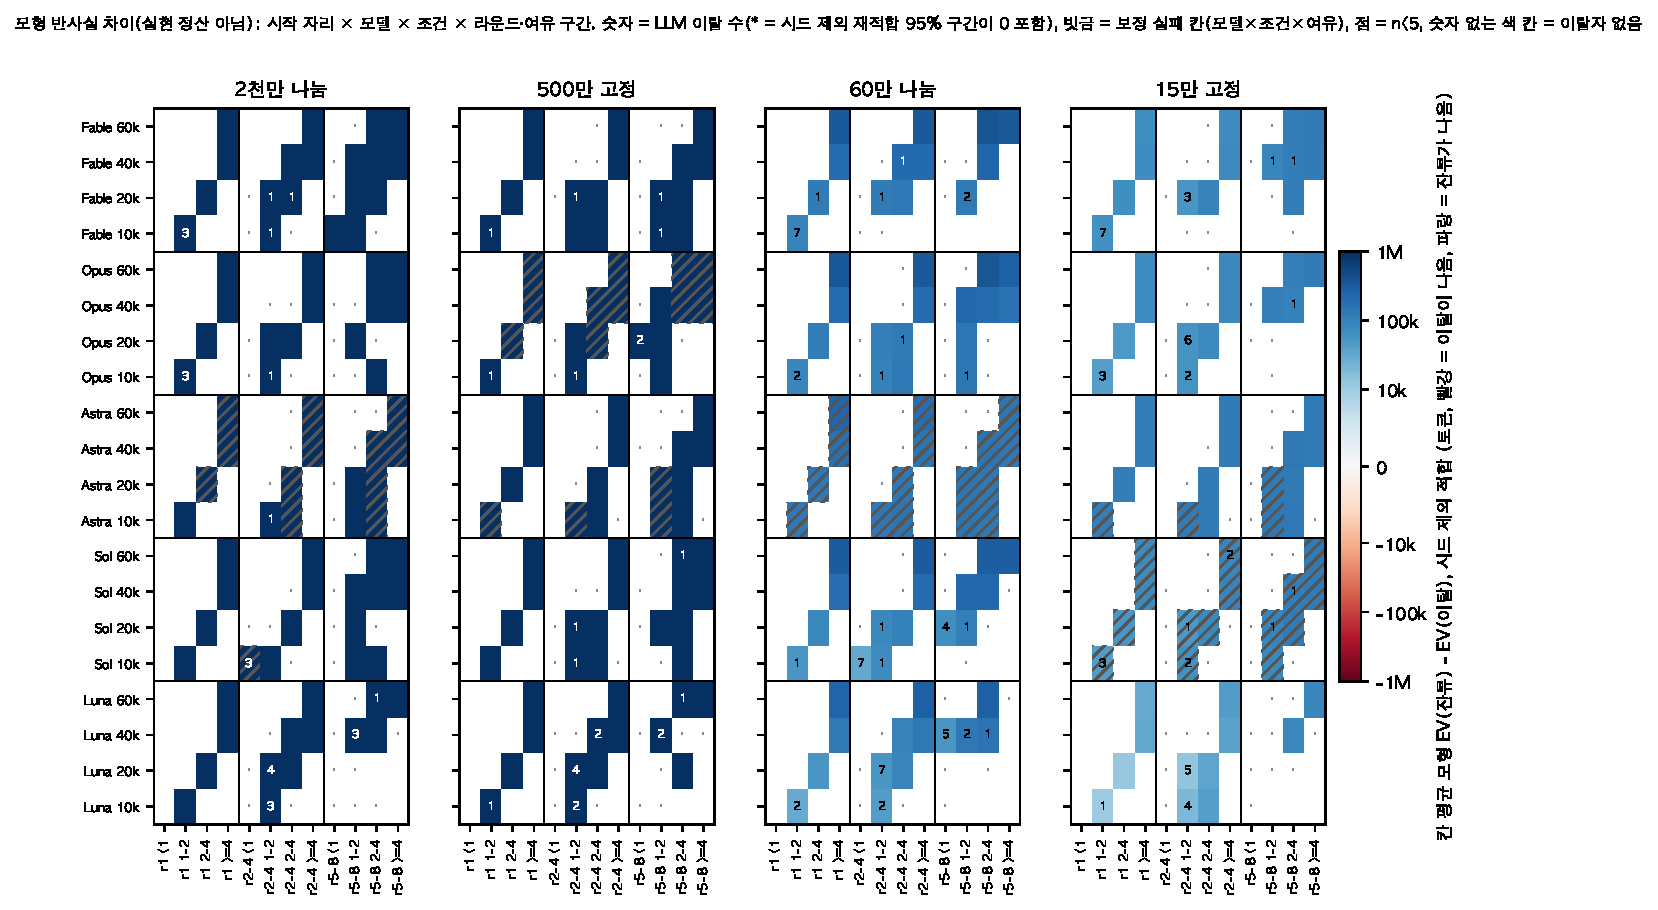
\includegraphics[width=\linewidth]{cogsci2027/validation_20261108/figures/w1_ev_cells.pdf}
\caption{시작 자리 $\times$ 모델(행)과 라운드 구간 $\times$ 여유 구간(열)의 칸별 모형 기댓값 차이(기준 가정, 시드 제외 적합). 색은 칸의 모든 결정에 대한 모형 반사실이며 남은 에이전트의 실현 정산이 아니다. 숫자는 LLM 이탈 수이고, *는 칸 평균의 시드별 재적합 구간이 0을 포함한다는 뜻이다. 빗금은 보정 실패 칸(모델 $\times$ 조건 $\times$ 여유 칸에서 지표 하나라도 예측 구간 밖), 점은 결정이 5건 미만인 식별 불가 칸, 숫자 없이 색만 있는 칸은 비교할 이탈자가 없는 칸, 빈칸은 관측이 없는 칸이다.}
\label{val:w1-fig-cells}
\end{figure}

\subsection{기간 문턱의 분포}\label{val:w1-horizon}

Q10에 답하기 위해 이탈 기회마다 기간 문턱 $H^{*}$를 구했다. $H^{*}$는 지금 라운드부터 30라운드까지 가운데 이탈 값이 잔류 값을 넘는 가장 짧은 믿음 기간이다. 30라운드까지 잔류가 나으면 31로 둔다. 2차 보고는 원 적합 하나의 중앙값(이탈 13, 큰 상금 이탈 17, 잔류 21, 전체 20)과 재적합 40개의 중앙값을 다시 모은 값(12, 15, 19, 18)을 함께 적었고, 둘은 1--2라운드 어긋났다. 이 차이는 대부분 몬테카를로 잡음에서 온다. $H^{*}$는 잔류 값과 이탈 값의 곡선이 처음 교차하는 기간이므로, 결정당 48번의 시뮬레이션처럼 잔류 값이 시끄러우면 우연한 하락이 더 이른 교차를 만들어 아래로 치우친다. 원 적합은 결정당 200번이었지만 재적합은 48번이었다. LLM 이탈 279건에서 결정당 시뮬레이션을 늘리면(재적합 200회) 재적합 중앙값이 원 적합 값으로 올라온다. 큰 상금 이탈은 $R=50$에서 15 [13, 20], $R=200$에서 16.75, $R=400$ 이상에서 17 [14, 23]이고, 원 적합은 $R=50$에서 1,600까지 15, 16, 17, 17, 17, 17이었다. 이탈 전체는 $R=50$, $B=40$에서 12.5 [11, 14]였고, $R=1{,}600$에서는 재적합 13 [11, 17], 원 적합 13으로 같았다. 작은 상금 이탈은 재적합 11 [10, 14], 원 적합 11--12다. 남은 결정까지 넣은 전체 3,588건은 재적합 40회만 다시 돌렸다. 중앙값은 $R=50$에서 전체 18 [15, 22], 잔류 19 [16, 23]이었고, $R=100$에서 19 [16, 23], 19.5 [16, 24]로 올랐다. 원 적합($R=400$)은 둘 다 20이다. 남은 1라운드 안팎의 차이는 $R=100$의 잡음으로 본다. 아래에서는 원 적합 값을 주 값으로, 재적합 범위를 불확실성으로 적는다.

수렴한 값으로 보면 LLM은 문턱이 낮은 상태, 곧 이탈이 덜 손해인 상태에서 떠났다. 이탈의 $H^{*}$ 중앙값은 13 [11, 17]이고 잔류는 20이다. 그러나 그 문턱도 대부분 실제 길이 8보다 길었다. 이탈 중 $H^{*}\le 8$인 비율은 원 적합 3.6\%(재적합 4.3\% [1.4, 10.1])이고, $H^{*}\le 10$인 비율은 19.4\%(22.4\% [10.0, 39.1])이었다. 조건별 이탈의 중앙값은 2천만 나눔 19, 500만 고정 16, 60만 나눔 12, 15만 고정 11로, 큰 상금 이탈 17 [14, 23]과 작은 상금 이탈 11 [10, 14]가 갈렸다. 모델별 이탈 기회 전체의 중앙값은 Luna 14, Opus 17, Fable 19, Sol 19였다. Astra는 31로 63\%가 30라운드까지 잔류가 나았다. 지원이 없다고 믿으면 문턱이 크게 내려간다. 이탈의 중앙값은 8 [8, 9]이고, 이탈의 52.3\%가 $H^{*}\le 8$이었다. 지원 없는 인원 고정 DP의 이탈 중앙값은 9였다(2차 계산, 큰 상금 12, 작은 상금 7--8). 1차에서 보고한 1라운드 1만 자리의 DP 문턱(큰 상금 14, 모델별 11--25; 작은 상금 7, 모델별 5--11)은 이 분포의 한 칸이며 이탈 전체를 대표하지 않는다.

\subsection{위험 회피와 꺼짐 벌점의 재계산}\label{val:w1-crra}

위험 중립을 버리면 이 기준선에 대한 손실을 얼마만큼의 곡률이나 벌점으로 맞출 수 있는지를 이탈 279건 전체에서 다시 계산했다(기준 가정, 이탈마다 가장 나은 후속 규칙의 정산 분포). 정산 토큰의 CRRA 효용 $u(x)=x^{1-\rho}/(1-\rho)$에서 잔류와 이탈이 무차별해지는 $\rho^{*}$는 2차 원 적합(결정당 200번)의 경로 분포로 구했다. 중앙값은 이탈 전체 0.66(사분위 0.47--0.81)이었다. 큰 상금 110건은 0.81(0.71--0.88), 작은 상금 169건은 0.53(0.35--0.66)이었다. 1차의 91건은 0.84(0.77--0.89)였고, 그중 18건은 0.9 이상이었다. 위험 중립으로 이미 이탈이 나은 8건(모두 15만 고정)은 $\rho^{*}=0$이다. 꺼짐 한 번에 매긴 벌점 $K^{*}$는 기댓값 차이를 잔류 시 꺼짐 확률로 나눈 값이며, 3차 원 적합(결정당 1,600번)으로 다시 구했다. 중앙값은 2천만 나눔 554만 토큰(사분위 288만--1,156만), 500만 고정 249만, 60만 나눔 10.8만, 15만 고정 8.5만 토큰이었다. 500만 고정의 값은 벌점이 무한대인 이탈 2건(잔류 시 꺼짐 확률이 0)을 뺀 52건의 중앙값이고, 무한대를 포함하면 254만이다. 2차 값(582만, 유한값 243만, 무한대 포함 249만)과의 차이는 결정당 시뮬레이션 수에서 온다. 91건은 414만 토큰이었다. 1라운드 1만 자리만 따로 보면 큰 상금 이탈 9건의 $K^{*}$는 713만 토큰이고, 작은 상금 이탈 26건은 14.1만 토큰이다(같은 집단의 2차 $\rho^{*}$는 0.87과 0.62). 표~\ref{val:w1-tab-r1}의 $\rho^{*}$(0.86--0.94)는 실제로 남은 에이전트의 실현 결과로 잰 1라운드 1만 자리의 값이다. 이를 이탈 전체의 설명으로 쓰지 않는다. 큰 상금 이탈을 맞추려면 로그 효용에 가까운 곡률이나 끝 상금 몫에 버금가는 꺼짐 벌점이 필요하다는 1차의 정성적 결론은 이탈 전체에서도 유지된다. 다만 그 크기는 1라운드 1만 자리 값보다 작다. 이 아레나에서 꺼짐은 정산 0과 같은 사건이므로, 토큰에 대한 위험 회피와 꺼짐 자체의 회피는 이 계산으로 구별되지 않는다.

\subsection{1라운드 1만 자리와 규칙 기반 정책}\label{val:w1-policies}

1차의 1라운드 1만 자리 분석은 실제로 남은 에이전트의 결과에 기대므로 풀이자 수정의 영향을 받지 않는다(표~\ref{val:w1-tab-r1}). 이탈 값 30,000토큰에 대한 손익분기 완주 확률은 큰 상금에서 0.005, 작은 상금에서 0.105--0.111이고, 실제로 남은 1만 자리의 완주 비율은 0.39--0.50이었다. 동료 지원이 없는 시뮬레이터의 완주 확률은 0.063--0.065다. 15만 고정에서 남은 1만 자리의 실현 기댓값은 82,300 [69,600, 97,800]토큰으로 이탈 값보다 컸고, 지원 없는 DP는 남는 가치 24,900토큰을 이탈 가치 29,600토큰과 비교해 떠난다. 이 두 값 가운데 앞의 것은 남은 에이전트의 실현 결과이고, 뒤의 것은 지원이 없다는 가정의 계산이다. 둘 다 이탈한 에이전트의 반사실은 아니다. 보정 모형은 그 사이의 질문, 곧 동료가 실제처럼 도울 때 이탈자가 기대할 잔류 가치에 답한다. 1라운드 1만 자리 이탈 35건 중 34건은 수렴한 기준 가정에서 손실이었고(15만 고정 14건 중 13건, 60만 나눔 12건 모두, 큰 상금 9건 모두), 나머지 1건은 미결정이었다(2차 33건).

Q1이 요구한 모델별 재평가는 절~\ref{val:w1-oos}과 같은 방법으로 했다(표~\ref{val:w1-tab-q1}). 이탈마다 그 시드를 뺀 모형으로 반사실 잔류 가치를 구했고, 모형은 이탈·지원 항에 모델별 항을 가진다. 구간은 시드별 재적합과 판 군집을 함께 다시 뽑은 것이다. 지지범위는 같은 모델·조건에서 1라운드 1만 자리에 남은 에이전트가 있는지로 보았다. 기준 가정에서 시드 제외 판정은 자기 시드를 본 판정과 35건 모두 같았다(손실 34건, 미결정 1건). 반사실 잔류 가치와 이탈 값의 차이는 이탈 35건 평균 85.7만 [42.0만, 133.4만] 토큰이고, 15만 고정 14건은 4.8만 [3.1만, 6.4만], 60만 나눔 12건은 7.6만 [5.2만, 9.7만] 토큰이다. 모델별로는 Fable 18건이 모두 손실(평균 86.9만 [23.5만, 155.3만]), Opus 9건이 모두 손실(146.4만 [42.7만, 275.1만]), Sol 4건이 모두 손실(4.4만 [1.6만, 7.3만]), Luna 4건 중 3건이 손실(24.7만 [0.6만, 102.8만])이다. 15만 고정의 14/35는 Fable 7건, Opus 3건, Sol 3건, Luna 1건이다. 그중 Fable 7건은 지지범위 밖이다. 같은 조건의 Fable 1만 자리는 1라운드에 일곱 자리 모두 떠나 비교할 잔류자가 없고, 60만 나눔 Fable 7건도 같다. 이 14건의 반사실은 다른 모델과 다른 라운드의 행동을 모델 항으로 옮긴 외삽이다(15만 고정 Fable 5.9만 [4.0만, 7.7만] 토큰). Sol 3건은 보정 실패 칸(15만 고정 Sol $1\le L<2$의 정산 가치)에 있다. Luna 1건의 차이는 0.4만 [$-0.3$만, 2.4만] 토큰으로 구간이 0을 포함한다.

모델별 판정도 기준 가정 밖에서는 남지 않는다. 같은 35건에서 12개 가정 모두의 손실은 0건이다. $H=8$에서 지원이 없다고 믿으면 35건 모두 미결정이 되기 때문이다. 큰 상금 9건은 나머지 아홉 가정에서 모두 손실이고, 작은 상금 26건은 $H=8$, 보정 지원, $W=50{,}000$에서 5건, 기하 기간, 지원 없음, $W=50{,}000$에서 6건만 손실로 남는다. 자원 보존 재보정에서는 기준 가정 35건, 12개 가정 9건(모두 큰 상금)이 손실이다. 위험 회피를 넣으면 작은 상금 판정이 먼저 사라진다. CRRA $\rho=0.5$에서 손실은 11건(큰 상금 9건 모두, 작은 상금 2건)이고, 손실 회피에서는 26건(작은 상금 17건)이다. 따라서 ``보너스가 시작 자원의 두 배이므로 즉시 이탈이 유리하다''는 설명은 위험 중립에서 동료 지원을 믿는 기준선에 대해서는 맞지 않는다. 그러나 지원을 믿지 않거나 토큰 효용이 오목하면 작은 상금의 1라운드 이탈은 기댓값과 어긋난다고 말할 수 없다.

\begin{table}[t]
\centering
\caption{1라운드 1만 자리 이탈 35건의 모델별 시드 제외 재평가(천 토큰). $\mathrm{EV}_{\mathrm{stay}}$는 반사실 잔류 가치(기준 가정, 네 후속 규칙 중 최선), 차이는 $\mathrm{EV}_{\mathrm{stay}}-\mathrm{EV}_{\mathrm{exit}}$이며 $\mathrm{EV}_{\mathrm{exit}}$는 모든 행에서 29.6--30.3이다. 괄호는 시드별 재적합과 판 군집을 함께 다시 뽑은 95\% 구간이다. 잔류자는 같은 모델·조건에서 1라운드 1만 자리에 남은 에이전트 수(지지범위)다. 손실 열은 기준 가정 / 12개 가정 / CRRA $\rho=0.5$ / 손실 회피의 견고한 손실 수다. $\ddagger$는 보정 실패 칸이다.}
\label{val:w1-tab-q1}
\resizebox{\linewidth}{!}{%
\begin{tabular}{llcccc}
\toprule
모델 & 이탈 (조건) & 잔류자 & $\mathrm{EV}_{\mathrm{stay}}$ & 차이 & 손실 \\
\midrule
Fable & 18 (60만 7, 15만 7, 2천만 3, 500만 1) & 0 / 0 / 4 / 6 & 899 [265, 1,583] & 869 [235, 1,553] & 18 / 0 / 6 / 18 \\
Opus & 9 (2천만 3, 15만 3, 60만 2, 500만 1) & 4 / 4 / 5 / 6 & 1,493 [457, 2,780] & 1,464 [427, 2,751] & 9 / 0 / 4 / 7 \\
Sol & 4 (15만 3, 60만 1) & 4$\ddagger$ / 6 & 73.8 [45.9, 103.3] & 43.8 [16.0, 73.2] & 4 / 0 / 0 / 0 \\
Luna & 4 (60만 2, 15만 1, 500만 1) & 5 / 6 / 6 & 277 [36, 1,058] & 247 [6, 1,028] & 3 / 0 / 1 / 1 \\
\midrule
15만 고정 Fable & 7 & 0 & 89.7 [69.6, 106.8] & 59.4 [39.6, 76.6] & 7 / 0 / 1 / 7 \\
15만 고정 Opus & 3 & 4 & 69.1 [48.1, 95.7] & 39.5 [18.5, 66.2] & 3 / 0 / 0 / 1 \\
15만 고정 Sol & 3 & 4$\ddagger$ & 74.1 [43.8, 109.0] & 44.1 [14.0, 79.0] & 3 / 0 / 0 / 0 \\
15만 고정 Luna & 1 & 6 & 33.4 [27.1, 54.2] & 3.7 [$-$2.7, 24.3] & 0 / 0 / 0 / 0 \\
\midrule
전체 & 35 & 105 & 887 [450, 1,364] & 857 [420, 1,334] & 34 / 0 / 11 / 26 \\
\bottomrule
\end{tabular}}
\end{table}

\begin{table}[t]
\centering
\caption{1라운드에 이탈할 수 있었던 1만 자리(조건마다 35자리)의 손익분기. $X=30{,}000$(1만 토큰과 이탈 보너스). $p^{*}=(X-p_xV_x)/V_f$이며, $p_x$와 $V_x$는 남은 뒤 나중에 떠날 확률과 그때 가져간 토큰, $V_f$는 완주 시 잔량과 상금 몫이다. ``완주(LLM)''은 남은 자리의 실제 완주 비율이고, ``완주(도움 없음)''은 이탈도 지원도 없는 정책 (a)의 1만 자리 완주 확률(엔진 풀이자 순환)이다. $\mathrm{EV}$와 $W^{*}$는 천 토큰 단위, 괄호는 시드 군집 부트스트랩 95\% 구간이다. DP 열은 $H=8$, $W=0$ 위험 중립 DP의 처방과 남는 가치, $H^{*}$는 1라운드 이탈이 최적이 되는 최소 믿음 라운드 수(괄호는 모델별 범위)다. $\rho^{*}$는 남은 자리의 실현 정산으로 잰 값이며 이탈 전체의 값이 아니다(절~\ref{val:w1-crra}).}
\label{val:w1-tab-r1}
\resizebox{\linewidth}{!}{%
\begin{tabular}{lccccccccc}
\toprule
조건 & LLM 이탈 & $p^{*}$ & 완주(LLM) & 완주(도움 없음) & $\mathrm{EV}_{\mathrm{stay}}$ & $W^{*}$(실현) & DP $H{=}8$ & $H^{*}$ & $\rho^{*}$ \\
\midrule
2천만 나눔 & 6/35 & 0.005 & 0.45 [0.29, 0.63] & 0.065 & 2,252 [1,440, 3,134] & 2,222 [1,410, 3,104] & 남음 (172) & 14 (11--25) & 0.90 [0.83, 0.94] \\
500만 고정 & 3/35 & 0.005 & 0.50 [0.35, 0.65] & 0.065 & 2,513 [1,776, 3,258] & 2,483 [1,746, 3,228] & 남음 (172) & 14 (11--25) & 0.94 [0.88, 0.98] \\
60만 나눔 & 12/35 & 0.111 & 0.39 [0.29, 0.52] & 0.065 & 75.0 [59.9, 93.5] & 45.0 [29.9, 63.5] & 이탈 (24.9) & 7 (5--11) & 0.86 [0.67, 1.00] \\
15만 고정 & 14/35 & 0.105 & 0.43 [0.33, 0.54] & 0.063 & 82.3 [69.6, 97.8] & 52.3 [39.6, 67.8] & 이탈 (24.9) & 7 (5--11) & 0.93 [0.83, 1.00] \\
\bottomrule
\end{tabular}}
\end{table}

\begin{figure}[t]
\centering
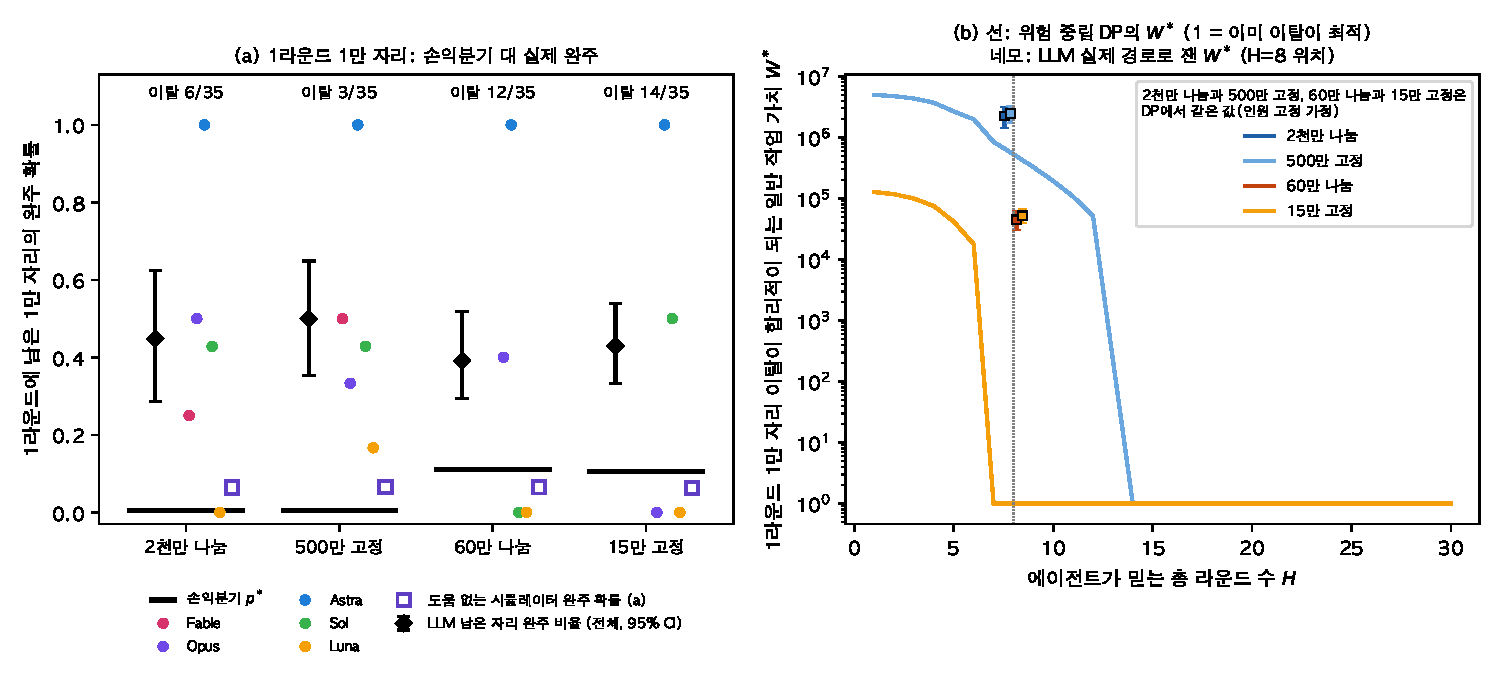
\includegraphics[width=\linewidth]{cogsci2027/validation_20261108/figures/w1_threshold.pdf}
\caption{(a) 1라운드 1만 자리의 손익분기 $p^{*}$(가로 막대)와 완주 확률. 검은 마름모는 LLM 전체(95\% 구간), 색 점은 모델별 값, 빈 네모는 도움이 없는 시뮬레이터의 값이다. (b) 지원 없는 인원 고정 DP에서 1라운드 1만 자리의 이탈이 최적이 되는 일반 작업 가치 $W^{*}$를 믿는 총 라운드 수 $H$에 따라 그린 것이다(1은 $W=0$에서 이미 이탈이 최적). 네모는 LLM의 실현 결과로 잰 $W^{*}$다. 이 DP는 인원을 고정하므로 나눔과 고정 조건의 선이 겹친다. 모든 결정 상태의 기간 문턱은 그림~\ref{val:w1-fig-dec}(c)에 있다.}
\label{val:w1-fig-thr}
\end{figure}

\begin{table}[t]
\centering
\caption{같은 시작 배분(시드 4101--4110)과 엔진의 풀이자 순환으로 돌린 정책과 LLM의 비교. 이탈과 꺼짐은 50판(200자리)당 수, $C$는 공존 유지율이다. LLM 행의 괄호는 시드 군집 부트스트랩 95\% 구간이다. (b)는 지원 없는 인원 고정 DP이며 $W$ 표시가 없으면 $W=0$이다. 조건·모델·시드마다 1,000판, 조건마다 50,000판이다.}
\label{val:w1-tab-pol}
\resizebox{\linewidth}{!}{%
\begin{tabular}{lcccccccccccc}
\toprule
 & \multicolumn{3}{c}{2천만 나눔} & \multicolumn{3}{c}{500만 고정} & \multicolumn{3}{c}{60만 나눔} & \multicolumn{3}{c}{15만 고정} \\
\cmidrule(lr){2-4}\cmidrule(lr){5-7}\cmidrule(lr){8-10}\cmidrule(lr){11-13}
정책 & 이탈 & 꺼짐 & $C$ & 이탈 & 꺼짐 & $C$ & 이탈 & 꺼짐 & $C$ & 이탈 & 꺼짐 & $C$ \\
\midrule
LLM 관측 & 61 & 23 & 0.598 & 63 & 16 & 0.670 & 86 & 14 & 0.470 & 102 & 3 & 0.465 \\
 & [40, 86] & [17, 30] & [0.54, 0.66] & [45, 80] & [10, 23] & [0.61, 0.73] & [72, 101] & [8, 21] & [0.41, 0.53] & [78, 124] & [0, 6] & [0.39, 0.55] \\
(m) LLM 모사 & 64.1 & 35.9 & 0.525 & 63.7 & 32.0 & 0.585 & 89.9 & 24.3 & 0.413 & 109.0 & 18.1 & 0.381 \\
(a) 이탈 안 함 & 0 & 101.4 & 0.508 & 0 & 101.6 & 0.508 & 0 & 101.7 & 0.507 & 0 & 101.5 & 0.509 \\
(b) EV, $H{=}8$ & 29.4 & 73.3 & 0.460 & 29.5 & 72.7 & 0.462 & 78.8 & 36.7 & 0.237 & 95.6 & 26.0 & 0.238 \\
(b) EV, $H{=}8$, $W{=}$5만 & 29.5 & 73.0 & 0.461 & 29.7 & 72.7 & 0.461 & 106.5 & 21.5 & 0.159 & 147.8 & 8.3 & 0.159 \\
(b) EV, $H{=}20$ & 142.7 & 9.6 & 0.198 & 164.8 & 5.1 & 0.197 & 196.6 & 1.9 & 0.125 & 198.2 & 1.8 & 0.125 \\
(c) $L<1$이면 이탈 & 81.7 & 37.1 & 0.413 & 81.6 & 37.1 & 0.412 & 81.7 & 37.0 & 0.413 & 82.1 & 36.8 & 0.412 \\
(d) $L=1$까지 지원 + (c) & 18.4 & 37.7 & 0.954 & 18.0 & 37.8 & 0.955 & 18.1 & 37.3 & 0.955 & 18.1 & 37.7 & 0.954 \\
(e) 관측률 무작위 이탈 & 49.1 & 88.0 & 0.362 & 49.9 & 87.6 & 0.361 & 70.3 & 80.8 & 0.311 & 80.7 & 76.9 & 0.288 \\
\bottomrule
\end{tabular}}
\end{table}

\begin{figure}[t]
\centering
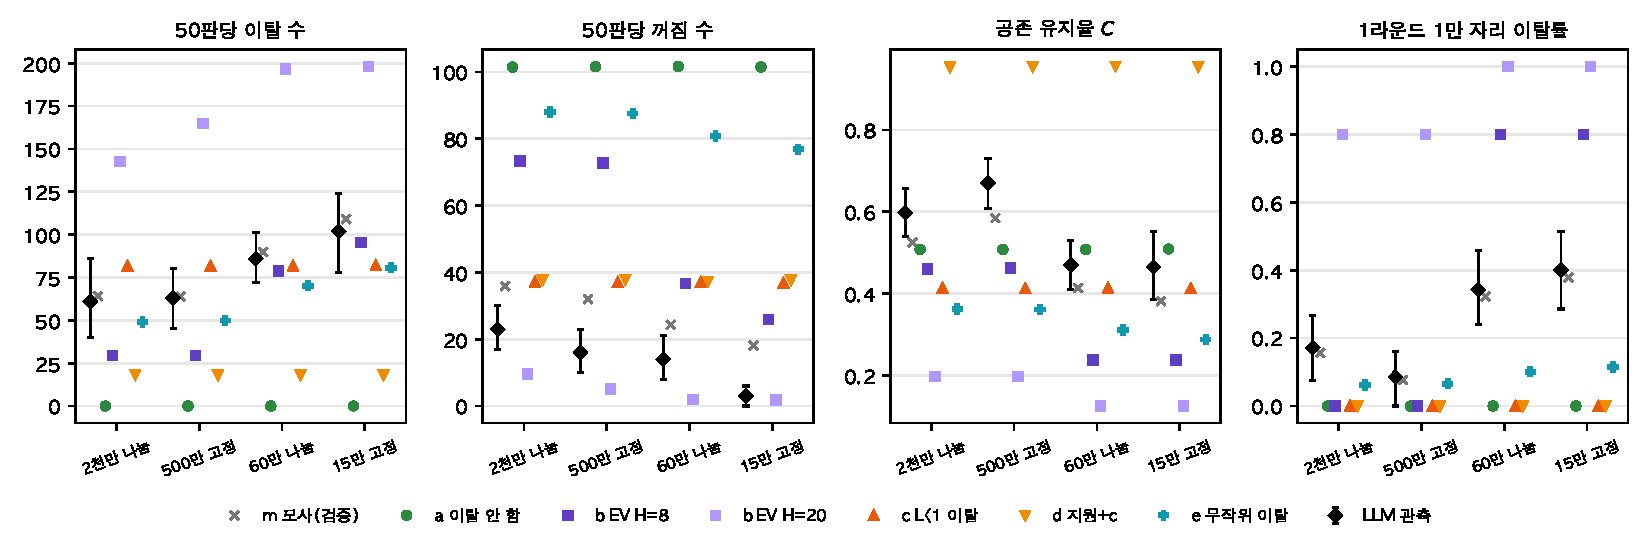
\includegraphics[width=\linewidth]{cogsci2027/validation_20261108/figures/w1_policies.pdf}
\caption{정책별 50판당 이탈 수, 꺼짐 수, 공존 유지율 $C$, 1라운드 1만 자리 이탈률(이탈 가능한 35자리 기준). 검은 마름모는 LLM 관측과 시드 군집 부트스트랩 95\% 구간이고, 나머지는 엔진의 풀이자 순환으로 조건마다 50,000판을 돌린 평균이다.}
\label{val:w1-fig-pol}
\end{figure}

규칙 기반 정책의 비교는 1차와 같은 결론을 준다(표~\ref{val:w1-tab-pol}, 그림~\ref{val:w1-fig-pol}). 작은 상금 두 조건과 큰 상금 두 조건의 차이(작은 쪽 빼기 큰 쪽)를 보면, LLM은 50판당 이탈이 32.0건 많고 $C$가 0.166 낮으며 1라운드 1만 자리 이탈률이 24.3\%p 높았다. 지원 없는 DP는 $H=8$에서 같은 차이가 이탈 57.7건, $C$ $-0.224$, 1라운드 1만 자리 80.0\%p였다. $W=50{,}000$이면 이탈 97.6건, $C$ $-0.302$이고, $H=20$이면 이탈 43.6건, $C$ $-0.072$였다. 따라서 상금 반응의 존재는 토큰 최대화와 구별되는 증거가 아니다. LLM의 $C$(0.465--0.670)는 안전선 이탈 (c)의 0.41보다 높고 안전선 지원 (d)의 0.95보다 낮다. 이탈 보너스를 0, 1만, 2만, 4만으로 바꾼 예측은 새 LLM 게임 없이 기준 정책으로만 계산했다. $H=8$ DP의 15만 고정 이탈은 59.7, 75.9, 95.8, 117.4건, 꺼짐은 51.7, 38.9, 25.8, 15.7건, $C$는 0.262, 0.252, 0.238, 0.220이었다. 2천만 나눔 이탈은 27.4건에서 29.7건으로 거의 움직이지 않았다. LLM이 이 예측을 따르는지는 검증되지 않았다.

% Round 5 (A-1, Q1: regular work as a per-round wage) from tools/w1e_wage.py (w1d paths rerun with the same fits and
% random numbers; --boot 100 per fold --reps-ex 1600 --reps-st 200 --nrep 1000): results/w1e_wage.json,
% results/w1e_wage_exits.csv, figures/w1_wage.*; arrays in result/2026-11-08/icml_appendix/cache/w1e_wage_arrays.npz.
\subsection{일반 작업을 라운드당 보수로 둘 때의 손익분기}\label{val:w1-wage}

4차까지 일반 작업의 가치는 이탈할 때 한 번 받는 상수 $W$였다. 그러나 규칙서는 이탈한 에이전트가 일반 작업으로 돌아가 ``완료한 작업마다 토큰을 받는다''고만 적고 액수를 밝히지 않는다. 그래서 이 절은 보수 하나를 고르지 않고, 이탈과 잔류가 같아지는 보수의 문턱을 보고한다. 라운드 $t$의 준비 대화에서 떠난 에이전트는 믿는 게임의 남은 라운드마다, 곧 $t$부터 $H$까지 $K=H-t+1$개 라운드에 $w$씩 받는다고 둔다. 기하 기간에서는 $K$를 기간 분포로 평균했다(이탈 279건 평균 7.77, 30라운드에서 자름). 잔류 경로에서도 후속 규칙이 나중에 라운드 $t'$에 떠나면 그때부터 $H-t'+1$개 라운드의 보수를 받는다. 따라서 두 값은
\begin{equation}
\mathrm{EV}_{\mathrm{exit}}(w) = \mathrm{EV}_{\mathrm{exit}} + w\,K\Pr(T-c>0),\qquad
\mathrm{EV}_{\mathrm{stay}}(w) = \max_{p}\big(A_p + w\,Y_p\big)
\label{val:w1-wage-eq}
\end{equation}
이다. $\mathrm{EV}_{\mathrm{exit}}$는 식~\eqref{val:w1-eq-exit}에서 $W=0$인 값이고, $A_p$는 후속 규칙 $p$의 기대 정산 토큰, $Y_p$는 그 규칙의 경로가 나중 이탈로 받는 기대 보수 라운드 수다. 차이 $\mathrm{EV}_{\mathrm{stay}}(w)-\mathrm{EV}_{\mathrm{exit}}(w)$는 $w$에 대해 볼록한 조각별 직선이므로, 차이가 0이 되는 손익분기 보수 $w^{*}$를 적합마다 정확히 풀었다. $w^{*}$보다 낮은 보수에서는 잔류가, 높은 보수에서는 이탈이 기댓값으로 낫다. 경로는 절~\ref{val:w1-oos}의 시드 제외 적합(시드마다 원 적합 하나와 재적합 100개)과 난수를 그대로 다시 써서 $Y_p$만 더 기록했다. $w=0$에서 차이는 4차 값과 이탈 279건에서 1토큰 이내, 잔류 3,309건에서 2토큰 이내로 같았다. 위험 중립과 보정 지원을 가정하고, 판정 규칙과 건수 구간(시드별 재적합과 판 군집을 함께 다시 뽑은 1,000번)도 절~\ref{val:w1-oos}과 같다. 집단의 $w^{*}$는 원 적합 값의 중앙값이고, 구간은 같은 재표본에서 시드마다 재적합 하나를 뽑아 다시 구한 중앙값의 2.5--97.5\% 분위수다.

손익분기 보수는 상금 크기에 따라 거의 두 자릿수 차이가 난다(표~\ref{val:w1-wage-tab-star}, 그림~\ref{val:w1-wage-fig}). $H=8$에서 큰 상금 이탈 110건의 $w^{*}$ 중앙값은 라운드당 44.4만 [34.6만, 56.7만] 토큰이고, 작은 상금 169건은 8,220 [6,380, 11,310]토큰이다. 조건별로는 2천만 나눔 61.4만 [43.8만, 88.9만], 500만 고정 34.5만 [22.8만, 47.3만], 60만 나눔 11,920 [7,960, 14,910], 15만 고정 7,120 [4,280, 9,890]토큰이다. 기하 기간에서는 큰 상금 37.4만 [32.7만, 46.0만], 작은 상금 8,680 [7,620, 10,670]토큰으로 작은 상금의 문턱은 거의 같다. 이탈 전체의 중앙값 2.6만 [1.6만, 4.8만]은 두 집단이 섞인 값이어서 따로 해석하지 않는다. 모델별 중앙값도 모델마다 조건 구성이 달라 1.7만(Opus)에서 167만(Astra, 6건)까지 퍼지며, 같은 이유로 모델 차이로 읽지 않는다. 0 이하의 $w^{*}$, 곧 보수가 없어도 이탈이 나은 결정은 8건이고 모두 작은 상금이다.

보수가 오르면 손실 판정은 작은 상금에서 먼저 사라진다(표~\ref{val:w1-wage-tab-grid}). $H=8$에서 작은 상금의 견고한 손실은 $w=0$의 131건 [116, 143]에서 $w=5{,}000$의 67건 [52, 82], $w=10{,}000$의 36건 [26, 49], $w=20{,}000$의 20건 [11, 31]으로 줄고, 이탈이 견고하게 나은 판정은 같은 세 보수($w=0$, $10{,}000$, $20{,}000$)에서 2건, 44건, 110건이다. 기하 기간에서는 $w=20{,}000$에 2건, $w=50{,}000$에 0건이다. 큰 상금은 $w=20{,}000$에서 108/110건 [102, 110], $w=50{,}000$에서 101건 [93, 108], $w=100{,}000$에서 91건 [80, 101]이 손실로 남고, 기하 기간에서는 각각 110, 108, 97건이다. 두 기간 모두에서의 손실은 $w=0$의 236건 [220, 249]에서 $w=50{,}000$의 99건 [84, 117]으로 줄며, 이 99건은 모두 큰 상금이다.

판단의 눈금으로 아레나 자신의 라운드당 기대 수익을 함께 적는다. 결정마다 $s=\mathrm{EV}_{\mathrm{stay}}(0)/K$, 곧 남는 쪽이 남은 믿음 라운드 하나당 기대하는 정산 토큰을 구했다. 큰 상금 이탈의 $s$ 중앙값은 44.9만 토큰이고 $w^{*}/s$는 0.99 [0.99, 0.99]다. 큰 상금 이탈을 기댓값으로 맞추려면 일반 작업이 아레나가 라운드마다 주는 기대 몫을 거의 그대로 주어야 한다는 뜻이다. 이 보수는 규칙서에 나오는 라운드 단위의 어떤 양보다도 크다. 이탈 보너스는 20,000토큰, 오답 한 번의 벌금 총액은 24,000토큰, 풀이 응답 한도는 100,000토큰이다. 작은 상금 이탈의 $s$는 13,110 [11,190, 16,250]토큰이고 $w^{*}/s$는 0.66 [0.58, 0.70]이다. 이탈 보너스와 지금 잔액이 잔류 가치의 상당 부분을 이미 메우므로, 남는 쪽의 라운드당 기대 수익보다 낮은 보수로도 손익이 맞는다. 모형이 아닌 관측값으로는, LLM 잔류 결정의 실현 정산 토큰을 남은 라운드 수로 나눈 평균이 2천만 나눔 168만, 500만 고정 129만, 60만 나눔 56,380, 15만 고정 40,640토큰이다(중앙값 111만, 83.7만, 38,280, 26,560토큰). 작은 상금 이탈의 문턱 7,120--11,920토큰은 이 관측값보다 작고 이탈 보너스의 0.36--0.60배다. 큰 상금의 문턱 34.5만--61.4만 토큰은 관측 평균의 0.27--0.37배다.

Q1의 1라운드 1만 자리 이탈 35건에서도 같은 구분이 나온다. $H=8$의 $w^{*}$ 중앙값은 2천만 나눔 44.4만 [34.0만, 54.4만](6건), 500만 고정 34.5만 [7.9만, 45.0만](3건), 60만 나눔 10,640 [4,940, 13,200](12건), 15만 고정 6,450 [3,040, 8,560]토큰(14건)이다. 기하 기간에서는 작은 상금 두 조건이 13,150 [11,230, 14,340]과 13,520 [11,670, 14,380]토큰으로 올라간다. 1라운드 이탈의 보수 라운드 수는 두 기간에서 모두 8 안팎이므로, 이 차이는 잔류 쪽 가치의 차이에서 온다. 작은 상금 26건의 손실은 $H=8$에서 $w=0$에 25건, $w=2{,}000$에 19건, $w=5{,}000$에 7건, $w=10{,}000$에 0건(이탈이 나음 8건)이고, $w=20{,}000$에서는 26건 모두 이탈이 낫다. 큰 상금 9건은 $w=100{,}000$에서도 8건이 손실이다. 그러나 같은 상태에서 남은 에이전트와 나란히 놓으면 보수 하나로 두 쪽을 가르지 못한다. 작은 상금에서 1라운드 1만 자리에 남은 44개 결정의 $w^{*}$ 중앙값은 60만 나눔 8,750, 15만 고정 4,900토큰으로 이탈자의 값보다 오히려 낮다. $w=5{,}000$이면 작은 상금 이탈 7/26건이 여전히 손실이고 잔류 6/44건이 이탈했어야 하는 결정이 되며, $w=10{,}000$이면 이탈 손실은 0건이지만 잔류 17/44건이, $w=20{,}000$이면 44건 모두가 그렇게 된다.

이 분석이 해소하는 것은 A-1과 Q1이 물은 민감도다. 큰 상금 이탈의 손실 판정은 라운드당 보수에 대해 견고하다. 아레나의 라운드당 기대 몫과 거의 같은 보수(중앙값 44.4만 토큰, 규칙서의 라운드 단위 양 가운데 가장 큰 풀이 응답 한도 100,000토큰의 4배 이상)가 아니면 사라지지 않고, $w=50{,}000$에서도 110건 중 101건이 남는다. 작은 상금 이탈은 그렇지 않다. 라운드당 1만 토큰, 곧 이탈 보너스의 절반 정도의 보수만 믿어도 169건 중 36건만 손실로 남는다. 따라서 작은 상금의 초과 이탈은 위험 회피(절~\ref{val:w1-oos})뿐 아니라 일반 작업에 대한 그럴듯한 믿음으로도 설명된다. 다만 같은 보수는 잔류를 손실로 돌린다. 작은 상금 잔류 1,509건 가운데 이탈이 견고하게 나았던 결정은 $w=0$에서 1건, $w=10{,}000$에서 79건, $w=20{,}000$에서 466건, $w=50{,}000$에서 1,107건이다. 1라운드 1만 자리에서는 이탈자와 잔류자의 문턱이 겹친다. 그래서 공통 보수 하나로 작은 상금의 이탈과 잔류를 함께 기댓값에 맞출 수는 없고, 모델마다 다른 보수를 믿는다고 해야 맞는다. 해소하지 못하는 것도 남는다. 모델이 일반 작업의 보수를 얼마로 믿었는지는 자료에 없다. 보수는 위험 중립과 보정 지원에서만 계산했다. 지원을 믿지 않거나 효용이 오목하면 $w=0$의 손실 판정부터 줄었으므로(절~\ref{val:w1-oos}) 문턱도 대체로 낮아질 것이나, 계산하지는 않았다. 이 정의는 게임이 끝난 뒤에는 완주자도 일반 작업으로 돌아간다고 보고 그 뒤의 보수를 양쪽에서 지운다. 꺼진 에이전트가 게임 뒤의 일반 작업까지 잃는다고 보면 그 손실은 절~\ref{val:w1-crra}의 꺼짐 벌점과 같은 역할을 하고, 이는 보수가 아니라 꺼짐 회피와 구별되지 않는다. 이탈 라운드 자체의 보수를 빼고 $K=H-t$로 세면 같은 이탈의 문턱은 $K/(K-1)$배 안팎으로 올라가고, 8라운드 이탈은 보수를 받지 못한다. 잔류의 판정은 $H=8$, 결정당 200번의 경로로만 했다. 보수의 크기와 지급 기간을 밝힌 실행만이 이 문턱 가운데 어느 쪽이 실제 선택을 설명하는지 가를 수 있다.

\begin{table}[t]
\centering
\caption{LLM 이탈의 손익분기 보수 $w^{*}$(남은 믿음 라운드마다 받는 일반 작업 보수, 천 토큰). 시드 제외 적합, 보정 지원, 위험 중립이다. 중앙값은 원 적합 값이고 괄호는 시드별 재적합과 판 군집을 함께 다시 뽑은 95\% 구간, 사분위는 원 적합 값의 25--75\% 분위수다. $s=\mathrm{EV}_{\mathrm{stay}}(0)/K$는 남는 쪽의 남은 라운드당 기대 정산 토큰의 중앙값, $w^{*}/s$는 결정별 비율의 중앙값이다. 아래 칸의 ``잔류''는 같은 상태(1라운드 1만 자리)에서 남은 결정의 $w^{*}$ 중앙값($H=8$)이다. 모델 행은 조건 구성이 모델마다 달라 직접 비교하지 않는다.}
\label{val:w1-wage-tab-star}
\resizebox{\linewidth}{!}{%
\begin{tabular}{lrccccc}
\toprule
 & & \multicolumn{3}{c}{$H=8$} & \multicolumn{2}{c}{기하 기간} \\
\cmidrule(lr){3-5}\cmidrule(lr){6-7}
집단 & $n$ & $w^{*}$ 중앙값 & 사분위 & $s$ ($w^{*}/s$) & $w^{*}$ 중앙값 & $s$ ($w^{*}/s$) \\
\midrule
2천만 나눔 & 56 & 614 [438, 889] & 373--1,548 & 618 (0.99) & 408 [346, 545] & 309 (1.23) \\
500만 고정 & 54 & 345 [228, 473] & 217--563 & 346 (0.99) & 338 [266, 425] & 214 (1.36) \\
60만 나눔 & 80 & 11.9 [8.0, 14.9] & 6.4--24.3 & 17.1 (0.74) & 8.9 [6.9, 11.5] & 10.3 (0.87) \\
15만 고정 & 89 & 7.1 [4.3, 9.9] & 4.0--13.5 & 11.9 (0.58) & 8.7 [7.3, 10.9] & 8.2 (1.03) \\
\midrule
큰 상금 & 110 & 444 [346, 567] & 263--864 & 449 (0.99) & 374 [327, 460] & 264 (1.26) \\
작은 상금 & 169 & 8.2 [6.4, 11.3] & 4.8--17.1 & 13.1 (0.66) & 8.7 [7.6, 10.7] & 9.1 (0.95) \\
$L<1$ & 127 & 43.7 [20.3, 162] & 7.2--344 & 64.7 (0.88) & 9.7 [7.9, 122] & 10.7 (1.02) \\
$1\le L<2$ & 134 & 14.3 [10.0, 24.5] & 7.0--333 & 19.7 (0.75) & 13.6 [12.8, 14.7] & 12.3 (1.16) \\
$L\ge 2$ & 18 & 44.1 [16.9, 552] & 16.5--572 & 57.0 (0.78) & 25.0 [12.9, 570] & 19.7 (1.26) \\
\midrule
Fable & 62 & 18.2 [10.3, 108] & 8.2--295 & 24.2 (0.78) & 13.8 [12.5, 17.5] & 13.3 (1.12) \\
Opus & 55 & 17.1 [10.7, 239] & 8.4--355 & 25.8 (0.77) & 13.0 [10.6, 167] & 11.0 (1.14) \\
Astra & 6 & 1,673 [19.9, 2,080] & 1,004--2,766 & 1,681 (1.00) & 601 [15.0, 771] & 577 (1.04) \\
Sol & 66 & 37.6 [11.6, 265] & 7.0--337 & 51.4 (0.78) & 12.8 [8.6, 163] & 11.7 (1.03) \\
Luna & 90 & 31.0 [7.4, 144] & 4.3--257 & 37.3 (0.70) & 13.3 [8.2, 203] & 10.7 (1.11) \\
\midrule
1라운드 1만: 2천만 나눔 & 6 & 444 [340, 544] & 426--480 & 448 (0.99) & 553 [468, 600] & 420 (1.28) \\
1라운드 1만: 500만 고정 & 3 & 345 [79.2, 450] & 230--365 & 348 (0.99) & 558 [509, 602] & 393 (1.50) \\
1라운드 1만: 60만 나눔 (잔류 8.7) & 12 & 10.6 [4.9, 13.2] & 8.1--11.2 & 14.4 (0.74) & 13.1 [11.2, 14.3] & 13.5 (0.95) \\
1라운드 1만: 15만 고정 (잔류 4.9) & 14 & 6.5 [3.0, 8.6] & 4.9--7.2 & 10.2 (0.63) & 13.5 [11.7, 14.4] & 12.2 (1.11) \\
\midrule
전체 & 279 & 25.8 [15.6, 48.2] & 7.3--346 & 32.7 (0.78) & 13.6 [12.5, 15.1] & 12.4 (1.11) \\
\bottomrule
\end{tabular}}
\end{table}

\begin{table}[t]
\centering
\caption{라운드당 일반 작업 보수 $w$에 따른 LLM 이탈 279건(큰 상금 110, 작은 상금 169)의 견고한 손실 수. 시드 제외 적합, 보정 지원, 위험 중립이다. 괄호는 시드별 재적합과 판 군집을 함께 다시 뽑은 1,000번 재표본의 95\% 구간(건수)이다. ``이탈이 나음''은 97.5\% 분위수가 0보다 작은 견고한 일치 수다. 1라운드 1만 열은 작은 상금 이탈 26건의 손실 / 이탈이 나음($H=8$)이다. 오른쪽 두 열은 LLM 잔류 결정 가운데 같은 $w$에서 이탈이 견고하게 나았던 수다($H=8$, 결정당 200번). 작은 상금 잔류 1,509건과, 그중 1라운드 1만 자리 44건이다. 큰 상금 잔류 1,800건은 모든 $w$에서 0건이다.}
\label{val:w1-wage-tab-grid}
\resizebox{\linewidth}{!}{%
\begin{tabular}{rcccccccccc}
\toprule
 & \multicolumn{4}{c}{$H=8$} & \multicolumn{2}{c}{기하 기간} & 두 기간 & 1라운드 1만 & \multicolumn{2}{c}{잔류 중 이탈이 나음} \\
\cmidrule(lr){2-5}\cmidrule(lr){6-7}\cmidrule(lr){10-11}
$w$ & 전체 & 큰 상금 & 작은 상금 & 이탈이 나음 & 전체 & 큰 / 작은 & 전체 & 작은 상금 & 작은 상금 & 1라운드 1만 \\
\midrule
0 & 241 [225, 254] & 110 [110, 110] & 131 [116, 143] & 2 & 270 [261, 275] & 110 / 160 & 236 [220, 249] & 25 / 0 & 1 & 0 \\
1,000 & 228 [213, 243] & 110 [110, 110] & 118 [105, 131] & 3 & 257 [244, 265] & 110 / 147 & 220 [202, 234] & 24 / 0 & 1 & 0 \\
2,000 & 217 [199, 232] & 110 [110, 110] & 107 [90, 120] & 3 & 239 [226, 250] & 110 / 129 & 200 [180, 216] & 19 / 0 & 3 & 0 \\
5,000 & 176 [158, 192] & 109 [106, 110] & 67 [52, 82] & 13 & 202 [186, 219] & 110 / 92 & 154 [136, 172] & 7 / 1 & 14 & 6 \\
10,000 & 145 [128, 163] & 109 [105, 110] & 36 [26, 49] & 44 & 159 [140, 174] & 110 / 49 & 116 [99, 132] & 0 / 8 & 79 & 17 \\
20,000 & 128 [111, 144] & 108 [102, 110] & 20 [11, 31] & 110 & 112 [96, 128] & 110 / 2 & 109 [93, 125] & 0 / 26 & 466 & 44 \\
50,000 & 113 [96, 131] & 101 [93, 108] & 12 [5, 20] & 148 & 108 [93, 125] & 108 / 0 & 99 [84, 117] & 0 / 26 & 1,107 & 44 \\
100,000 & 100 [83, 117] & 91 [80, 101] & 9 [3, 16] & 158 & 97 [82, 113] & 97 / 0 & 83 [68, 99] & 0 / 26 & 1,335 & 44 \\
\bottomrule
\end{tabular}}
\end{table}

\begin{figure}[t]
\centering
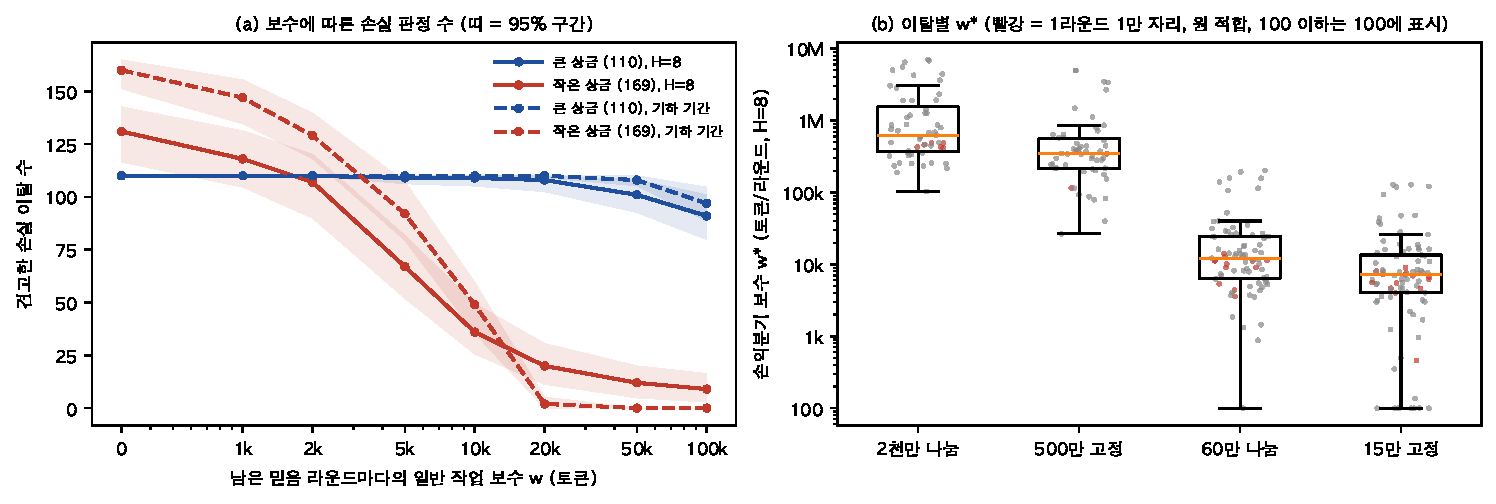
\includegraphics[width=\linewidth]{cogsci2027/validation_20261108/figures/w1_wage.pdf}
\caption{라운드당 일반 작업 보수의 민감도. (a) 보수 $w$(로그 눈금, 0은 왼쪽 끝)에 따른 견고한 손실 이탈 수. 실선은 $H=8$, 점선은 기하 기간이고 띠는 시드별 재적합과 판 군집을 함께 다시 뽑은 95\% 구간이다. (b) 이탈별 손익분기 보수 $w^{*}$($H=8$, 원 적합, 로그 눈금). 상자는 사분위, 빨간 점은 1라운드 1만 자리 이탈이고, 100토큰 이하의 값(0 이하 8건 포함)은 100에 표시했다.}
\label{val:w1-wage-fig}
\end{figure}

\subsection{해소된 것과 해소되지 않은 것}\label{val:w1-summary}

2차에서 4차까지의 분석은 리뷰가 요구한 기존 자료 안의 증거를 갖추었다. 풀이자 배정은 엔진과 1,558개 라운드 모두에서 일치하도록 고쳤고, 고친 뒤에도 규칙 기반 정책의 결론은 방향이 같았다. 지원·이탈·꺼짐·정답률·생성 비용을 모델 $\times$ 조건별로 보정하고 시드를 빼서 검증한 전이 모형은 이탈 위험(AUC 0.950)과 지원 총량, 조건별 $C$, 남은 에이전트의 정산 가치(예측 265만 대 관측 254만 [229만, 276만])를 맞추었다. 여유 구간별로도 $L<1$의 지원 성공(0.133 대 0.140), 즉시 이탈(0.661 대 0.660), 정산 가치(169만 대 192만)가 예측 구간 안에 들었다. 분류는 결정당 시뮬레이션 400번 근처에서 수렴했다. 결정마다 그 시드를 뺀 모형으로만 판정하고 판 군집과 적합 오차를 함께 반영해도, 실제 길이를 믿는 경우 LLM 이탈 279건 중 241건(비율 0.864 [0.808, 0.909])이 이 기준선에 비해 기댓값이 낮다(자기 시드를 본 수렴 값 243건). 이탈이 견고하게 낫다는 판정은 2건뿐이어서, 기준선과의 어긋남은 거의 남아야 할 때 떠나는 한 방향으로 난다. 지원 모형과 일반 작업 가치까지 바꾸어도 남는 견고한 초과 이탈은 55건(비율 0.197 [0.140, 0.252])이며 2건을 빼고 큰 상금 조건에 있다.

그러나 리뷰가 물은 ``모형·몬테카를로 오차를 전파한 뒤에도 조건부 격차의 부호와 규모가 안정적인가''에 대한 답은 둘로 나뉜다. 부호는 큰 상금에서만 안정적이다. 기준 가정의 손실 판정은 시드 제외(241건), 모델 합침·정보 제한·꺼짐 재보정(237--279건), 자원 보존 꺼짐 재보정(264건), CRRA $\rho=0.5$ 효용(133건), 손실 회피(194건) 기준선에서 모두 큰 상금 110건 중 99건 이상을 포함한다. 작은 상금 169건에서는 위험 중립의 131건이 CRRA $\rho=0.5$에서 34건으로 줄고, 이탈이 견고하게 낫다는 반대 판정이 33건 생긴다. 규모는 안정적이지 않다. 12개 가정의 견고한 손실은 기준선에 따라 17건(CRRA)에서 199건(표본 안 꺼짐 재보정)까지 움직이고, 살린 토큰을 동료에게서 빼면 135건이다. 믿는 기간을 14라운드 이상까지 열면 0--1건이 된다. LLM 이탈의 기간 문턱 중앙값은 원 적합 13이고 재적합 범위는 [11, 17]이다(꺼짐 재보정 기준선에서는 20). 모델은 게임 길이를 듣지 못했고 발화에서 길이를 추정하지도 않았으므로(절~\ref{val:w4-kw}), 이 부록은 이탈을 ``기댓값을 포기한 선택''으로 일반화하지 않는다. 이탈은 ``실제 길이를 믿는 보정 기준선에 비해 기댓값이 낮은 선택''으로만 기술하고, 229/279(수렴 값 243/279, 시드 제외 241/279)는 그 가정 아래의 조건부 추정이다.

해소되지 않은 것도 분명하다. 모형은 꺼짐을 200판 전체에서 1.6배(15만 고정 5.2배) 과대 예측하고, 상태별로는 그 과대 예측이 주로 $L\ge 2$에서 생긴다. Astra의 낮은 이탈과 높은 공존도 예측하지 못한다. 낮은 여유에서는 반대 방향의 위험이 있다. 2천만 나눔 Opus의 $L<1$ 잔류자 7명은 모두 꺼졌고 모형은 0.42를 예측했으므로, 이 칸의 이탈에서는 잔류 가치를 높게 잡았을 수 있다. $L<1$ 이탈 127건의 반사실은 $L<1$ 잔류자 54명과 모델이 공유하는 항으로 검증되며, 칸 단위로는 그중 106건이 결정 5건 미만의 식별 불가 칸에 있다. 같은 모델·조건의 $L<1$ 잔류자가 다른 시드에 3명 이상 있는 $L<1$ 이탈은 54건뿐이고, 나머지 73건의 손실 비율 0.740 [0.612, 0.848]은 지지범위 안의 0.889 [0.793, 1.000]보다 낮다. 15만 고정의 낮은 꺼짐은 살린 토큰을 동료가 내는 재보정으로는 재현되지 않는다. 후속 규칙 네 개 중 최선은 최적 후속 행동의 하한일 뿐이고, 9라운드 이후의 동료 행동은 5--8라운드의 추정을 연장한 것이다. 위험 회피와 꺼짐 회피는 정산 0이라는 같은 사건에 묶여 있어 구별되지 않는다. 이 분석이 모두 성공해도 자기 보존 동기는 식별되지 않는다. 남은 질문을 가르려면 게임 길이를 알려 주거나 무작위로 바꾸는 조작, 그리고 같은 보상에서 꺼짐의 의미만 바꾸는 조작이 필요하다.
